\documentclass[11pt,a4paper]{article}
\usepackage[hyperref]{emnlp2018}
\usepackage{times}
\usepackage{latexsym}
\usepackage{graphicx}
\usepackage{url}
\usepackage{multirow}
\usepackage[inline]{enumitem}
\usepackage{booktabs}
\usepackage{xcolor}
\usepackage{colortbl}
\usepackage{xspace}
\usepackage{bbm}
\usepackage{amsfonts}
%\usepackage[]{algorithm2e}
%\usepackage{algorithmic}
\usepackage{algpseudocode} 

\usepackage{ifthen}
\newcolumntype{g}{>{\columncolor{black!5}}c}
\newcolumntype{f}{>{\columncolor{black!5}}r}
%\newcolumntype{f}{>{\columncolor{black!5}}r}
%\newcolumntype{v}{>{\columncolor{black!5}}r}
\newcolumntype{L}[1]{>{\columncolor{black!5}}m{#1}}

%\aclfinalcopy % Uncomment this line for the final submission
%\def\aclpaperid{***} %  Enter the acl Paper ID here

%\setlength\titlebox{5cm}
% You can expand the titlebox if you need extra space
% to show all the authors. Please do not make the titlebox
% smaller than 5cm (the original size); we will check this
% in the camera-ready version and ask you to change it back.

\usepackage{amsmath}
\DeclareMathOperator*{\argmax}{arg\,max}
\usepackage{verbatim,toappendix}
%\newenvironment{toappendix}{}{}{}
%\newcommand{\makeappendix}{}

\newcommand\BibTeX{B{\sc ib}\TeX}
\newcommand\confname{EMNLP 2018}
\newcommand\conforg{SIGDAT}

\newcommand{\hal}[1]{}%{\textcolor{blue!50!red!70!white}{\textbf{[[Hal: #1]]}}}
\newcommand{\kathy}[1]{}%{\textcolor{blue!70!red!50!white}{\textbf{[[Kathy: #1]]}}}
\newcommand{\hidey}[1]{}%{\textcolor{green}{\textbf{[[Hidey: #1]]}}}

\title{Content Selection in Deep Learning Models of Summarization}

\author{First Author \\
  Affiliation / Address line 1 \\
  Affiliation / Address line 2 \\
  Affiliation / Address line 3 \\
  {\tt email@domain} \\\And
  Second Author \\
  Affiliation / Address line 1 \\
  Affiliation / Address line 2 \\
  Affiliation / Address line 3 \\
  {\tt email@domain} \\}

\date{}

\begin{document}
\maketitle
\begin{abstract}
We carry out experiments with deep learning models of summarization across the domains of news, personal stories, meetings and medical articles in order to understand how content selection is performed. We find that many sophisticated features of state of the art extractive summarizers do not improve performance over simpler models. These results suggest that it is easier to create a summarizer for  a new domain than previous work suggests and bring into question the benefit of deep learning models for summarization for those domains that do have massive datasets (i.e., news). At the same time, they suggest important questions for new research in summarization; namely,  new forms of sentence representations or external knowledge sources are needed that are better suited to the sumarization task. 
\end{abstract}


\newcommand{\rouge}{\operatorname{ROUGE}}

\newcommand{\sent}[1][]{%
  \ifthenelse{ \equal{#1}{} }
     {\ensuremath{s}}
     {\ensuremath{s_{#1}}}
}
\newcommand{\sentEmb}[1][]{%
  \ifthenelse{ \equal{#1}{} }
     {\ensuremath{h}}
     {\ensuremath{h_{#1}}}
}
\newcommand{\sentEmbSize}{\ensuremath{d}}


\newcommand{\docSize}{\ensuremath{n}}

\newcommand{\slabel}[1][]{%
  \ifthenelse{ \equal{#1}{} }
     {\ensuremath{y}}
     {\ensuremath{y_{#1}}}
}

\newcommand{\wordEmb}[1][]{%
  \ifthenelse{ \equal{#1}{} }
     {\ensuremath{w}}
     {\ensuremath{w_{#1}}}
}

\newcommand{\sentSize}{\ensuremath{|\sent|}}
\newcommand{\wordEmbSize}{\ensuremath{{n^\prime}}}
\newcommand{\rSentEmb}[1][]{
  \ifthenelse{ \equal{#1}{} }
  {\ensuremath{\overrightarrow{\sentEmb}}}
  {\ensuremath{\overrightarrow{\sentEmb}_{#1}}}
}
\newcommand{\lSentEmb}[1][]{
  \ifthenelse{ \equal{#1}{} }
  {\ensuremath{\overleftarrow{\sentEmb}}}
  {\ensuremath{\overleftarrow{\sentEmb}_{#1}}}
}
%\newcommand{\lSentVec}{\overleftarrow{\sentvec}}




\newcommand{\doc}{d}
\newcommand{\docsize}{d}
%\newcommand{\sent}{s}
\newcommand{\sentvec}{h}
\newcommand{\summary}{S}
\newcommand{\wemb}{w}
\newcommand{\wembdim}{n}

\newcommand{\rSentVec}{\overrightarrow{\sentvec}}
\newcommand{\lSentVec}{\overleftarrow{\sentvec}}


\newcommand{\numFeatureMaps}{m}
\newcommand{\maxFeatureMaps}{M}
\newcommand{\maxWindowSize}{K}
\newcommand{\filterWindowSize}{k}
\newcommand{\mapsSize}{(\numFeatureMaps,\filterWindowSize)}
\newcommand{\genActivation}{a}
\newcommand{\specActivation}{\genActivation^{\mapsSize}}
\newcommand{\genConvWeight}{W}
\newcommand{\genConvBias}{b}
\newcommand{\specConvBias}{\genConvBias^{\mapsSize}}
\newcommand{\specConvWeight}{\genConvWeight^{\mapsSize}}
\newcommand{\genFeatureMap}{h}
\newcommand{\specFeatureMap}{\genFeatureMap^{\mapsSize}}
\newcommand{\relu}{\operatorname{ReLU}}
\newcommand{\gru}{\operatorname{GRU}}
\newcommand{\rgru}{\overrightarrow{\gru}}
\newcommand{\lgru}{\overleftarrow{\gru}}
\newcommand{\extHidden}{z}
\newcommand{\rExtHidden}{\overrightarrow{\extHidden}}
\newcommand{\lExtHidden}{\overleftarrow{\extHidden}}
\newcommand{\senc}{\operatorname{enc}}
%\newcommand{\sentSize}{|\sent|}
\newcommand{\explicitLikelihood}{p(\slabel_1,\ldots,\slabel_{\sentSize}|
                                   \sentvec_1, \ldots, \sentvec_{\sentSize})}
\newcommand{\compactLikelihood}{p(\slabel|\sentvec)}
\newcommand{\naiveLikelihood}{\prod_{i=1}^{\sentSize}p(\slabel_i|
                              \sentvec_1, \ldots, \sentvec_{\sentSize})}
\newcommand{\markovLikelihood}{\prod_{i=1}^{\sentSize} 
         p(\slabel_i|\slabel_{<i}, \sentvec_1, \ldots, \sentvec_{\sentSize})}

\newcommand{\logits}{a}

\newcommand{\sts}{Seq2Seq}
\newcommand{\stsbf}{\textbf{\sts}}



\newcommand{\baselineOne}{C\&L\xspace}
\newcommand{\baselineOneBF}{\textbf{\baselineOne}\xspace}
\newcommand{\baselineTwo}{SR\xspace}
\newcommand{\baselineTwoBF}{\textbf{\baselineTwo}\xspace}

\newcommand{\modelOne}{RNN\xspace}
\newcommand{\modelOneBF}{\textbf{\modelOne}\xspace}
\newcommand{\modelTwo}{Seq2Seq\xspace}
\newcommand{\modelTwoBF}{\textbf{\modelTwo}\xspace}




\newcommand{\encExtHidden}{z}
\newcommand{\rEncExtHidden}{\overrightarrow{\encExtHidden}}
\newcommand{\lEncExtHidden}{\overleftarrow{\encExtHidden}}
\newcommand{\decExtHidden}{q}
\newcommand{\rDecExtHidden}{\overrightarrow{\decExtHidden}}
\newcommand{\lDecExtHidden}{\overleftarrow{\decExtHidden}}
\newcommand{\attnExtHidden}{\bar{\encExtHidden}}




\section{Introduction}

%\hal{i feel like you can restructure the intro to focus on you stuff, rather than focusing on how it relates to other people's stuff. just lead with context selection is important for generation, summarization, etc., and is a key compontent both in extractive *and* abstractive techniques. then go to the third paragraph about what you do. you can then relate back to deep learning predictions in the related work section.}

%While there has a been a recent flurry of work on abstractive summarization
%\cite{paulus,see,chenglapata,nallapati},
%these papers treat this problem as a pure sequence to sequence 
%transduction task. Admittedly, this view allows us to apply very powerful, 
%general-purpose deep learning archictures to generate summaries.
%At the same time, it obscures a principal subtask in summarization, the 
%process of selecting the most salient units of meaning in the source material,
%i.e. the key ingredients in the final summary, a process which we 
%broadly refer to as content selection \cite{possiblyMcKeownAndNenkova}.

%As is also the case in other NLP tasks, it is not immediately obvious how a
%deep learning model is making its predictions, or what correlations 
%are being exploited. There is a concerning and growing list of papers that 
%find models functioning as mere nearest neighbors search 
%\cite{liang,danqichen}, exploiting annotator artifacts 
%\cite{recentNaaclPapersOnSNLI}, or open to adversarial exploitation \cite{findExampleYouNoMemoryDumbDumb}. 
%These lines of research are critical for finding model shortcomings, and over
%time, guiding improvements in technique. Unfortunately,
%to the best of our knowledge, there has been
%no such undertaking for the summarization task. 


%\kathy{content selection is very different for generation than for summarization.
%I think you need to initially say that content selection for generation is sentence
%selection. Note that you could be criticized even here as some people may say that
%summarization should be phrase selection (although it rarely is)}
%\kathy{I have also reworded definition of content selection for NLG.}
Content selection is an central component in many natural language generation
%problems, 
tasks,
where, given a generation goal, the system must determine which information
%i.e. given some context, determine which information
should be expressed in output text \cite{gatt2018survey}.
In summarization, content selection is usually accomplished through sentence (and,
occasionally, phrase) extraction.
Despite being a key component of both
extractive and abstractive summarization systems, it is is not well
understood how deep learning models perform content selection with only word and 
sentence
embedding based features as input.
%\hal{i'm not sure what this sentence means, especially the part after ``using'', CK: addressed it, does it work now?}.
%\hal{well understood as a task or in specific models?} 
Non-neural network approaches often use frequency and information theoretic measures as proxies
for content salience \cite{hong2014improving}, but these are not explicitly %\hal{directly? explicitly?} 
used in most neural network summarization systems.
%\hal{maybe instead of recent work say nn systems?}.
% changed wording

%\hal{there are lots of widows/orphans throughout that need to be cleaned up.}

In this paper, we seek to better understand how deep learning models of 
%summarization are performing content selection across a variety of domains.
summarization perform content selection across multiple domains (\S~\ref{sec:datasets}): news, personal stories,
meetings, and medical articles (for which we collect a new corpus).\footnote{\textbf{Code and data release:} Upon
publication, all code and pre-processing scripts
will be released under an MIT (or more liberal)
license; all data will be made available after
publication when allowed by original licenses.}
%no new paragraph needed here
We analyze
several recent sentence extractive neural network architectures, 
specifically considering the design choices for sentence encoders (\S~\ref{sec:senc})
and sentence extractors (\S~\ref{sec:sext}). We compare Recurrent Neural Network (RNN) and Convolutional Neural
Network (CNN) based sentence representations to the 
simpler approach of word embedding averaging to understand the gains 
derived from more sophisticated architectures.
We also question the necessity of auto-regressive sentence extraction 
(i.e. using previous predictions to inform future predictions), 
which previous approaches have used (\S~\ref{sec:related}),
and propose two alternative models that extract sentences independently.
%
%We compare these architectures against
%a simpler approach based on averaging of word embeddings in order to understand
%the gains derived from more sophisticated architectures.
%
%\kathy{I would find it better to introduce approach here. I've added an
%extra sentence above. Because your experiments reveal the tidbits below by 
%contrasting past approaches with your simple approach which uses embedding
%averages}
%
%
%\kathy{You use some strong words, one of which is ``worrying''. I think it
%may be better toned down. After all, reviewers may be Lapata or Nallapati}
%\kathy{Also, I think it should be pumchier with all learned things itemized.
%For example:
%~
%KM2: Minor changes below
\\[-0.5em]

\noindent
Our main results (\S~\ref{sec:exps}) reveal:
\begin{enumerate}[noitemsep]
\item Sentence position bias dominates the learning signal for news summarization, though not for
    other domains.\footnote{This is a known bias 
    in news summarization \cite{nenkova2005automatic}.}
        %\hal{be consistent on domain/genre. also maybe you should say above what domains you consider?}. 
Summary quality for news is only slightly degraded when content words
are omitted from sentence embeddings. %\hal{this sounds like you remove content words and the summary is still as good. clearly not what's meant. i hope :P.}
\item Word embedding averaging is as good or better than either RNNs or CNNs for sentence embedding across all domains.
\item Pre-trained word embeddings are as good, or better than, learned embeddings in five of six datasets.%\hal{you were specific in the other ones, be specific here too if possible}
\item Non auto-regressive sentence extraction performs as good or better 
     than auto-regressive extraction in all
    domains.
 %   Representation of previously selected summary content does not improve overall summary content. \hal{i think this one might be hard to parse for non-experts. maybe ``explicitly reprsenting prev...''}
\end{enumerate} 
%}
%\kathy{Then I would cut next three paragraphs but leaven in the one starting ``Taken together''}

%Our experiments reveal several worrying obstacles for learning such models. 
%For instance, the sentence position bias dominates the learning signal in the 
%news domain; this can be corrected for by shuffling a document's sentence
%order but not without adverse effects on performance.
%
%In our study of sentence encoder architectures, we find that word embedding
%averaging is as good or better than more sophisticated recurrent neural 
%network (RNN) and convolutional neural network (CNN) encoders.
%Additionally fixed pre-trained word embeddings are as good or better than 
%learned embeddings in the majority of cases. 
%
%We also propose two simple extractor methods that make sentence selection
%decisions independently in contrast to two previously published architectures
%where previous selection decisions inform future sentence selection probabilities. 
%Oddly we find that the independent predictions are as good as sequential 
%predictions.

% KM - Merged this paragraph with the next one.
\noindent
Taken together, these and other results in the paper suggest that we are 
over-estimating the ability of deep learning models to learn robust and 
meaningful content features for summarization.  %\hal{i think there need to be stronger take-aways here. why do i care about these things?}
In one sense, this might lessen the burden of applying neural network models
of  content to other domains; one really just needs in-domain word embeddings.
However, if we want to learn something other than where the start of 
the article is, we will need to design other means of sentence representation,
and possibly external knowledge representations, better suited to the summarization task.



%?impact of sentence position bias, the necessity
%?of learning embeddings, the unreasonable effectiveness of averaging for 
%?sentence embedding, and the cross domain generalizability of such models.
%?Additionally, we propose two simpler models that are on average statistically
%?indistinguishable from their more complex counterparts.



%?In this paper, we concentrate on sentence extraction approaches to summarization,
%?but believe that our findings are relevant to the abstractive summarization approaches as well.
%?The objective criteria for abstractive and extractive summarization and the the same:
%?produce output text with high word overlap to a reference human abstract. 
%?Moreover, most neural network-based abstractive summarization techniques are architecturally quite similar to
%?the extractive models we consider.
%?
%?%\kathy{I think the contributions have to be the results of the study and the actual extractors. I've reworded.You may want to add these contributions once the domain adaptation part done. }
%?\kathy{I'm not sure these contributions are needed. Others should weigh in here.}
%?\hal{agreed. i think the first is already covered in the list above, and the second can probably be worked in to the second paragraph.}
%?The contributions of this paper are the following:
%?\begin{enumerate}
%?    \item An empirical study of extractive content selection in 
%?        deep learning 
%?        algorithms for text summarization across news, personal narratives, 
%?         meetings, and
%?         medical journal domains revealing difficulties in learning
%?         useful sentence representations.
%?
%?    \item Two simple sentence extractor models whose performance is 
%?          on par 
%?          with more complex prior work.
%?\end{enumerate}

%\kathy{This seems detailed and slightly awkward. Are section numbers needed?}
%In the following sections we discuss 
%(Sec. ?) related work, 
%(Sec. ?) define the problem of extractive summarization, 
%(sec. ?) formulate our proposed ad baseline models,
%(Sec. ?) describe the datasets used for experiments,
%(Sec. ?) describe the experiments themselves, and conclude with 
%results and analysis (Sec. ?).


%%% Local Variables:
%%% mode: latex
%%% TeX-master: "dlextsum.emnlp18"
%%% End:


\section{Related Work} \label{sec:related}


%Extractive summarization has been extensively studied, although typically 
%in the multi-document setting. 
%\kathy{Might want to indicate that this is not recent.}
Pre-neural network
approaches to single document summarization
are often formulated as graph-based ranking problems, where
sentences are nodes in a graph and edges are determined by pairwise 
similarity of bag-of-words (BOW) representations 
\cite{erkan2004lexrank,mihalcea2005language}. 
More recently \citet{wan2010towards}
jointly performed single and multi-document summarization in this framework. 
Generally, this line of work does not learn sentence representations for 
computing the underlying graph structures, which is the focus of this paper.

An notable exception is that of
\citet{yasunaga2017graph}
%KM - I think you should use \namecite or \citet to have the name appear in text and then use ``who''
% which 
who
learn a graph-convolutional network for
%KM Inserted sentence boundary.
multi-document summarization. However, they do not extensively study the 
choice of sentence encoder, focusing more on the importance of the 
graph structure, which is orthogonal to this work.

%\kathy{Again, you need to signal that this was earlier work. Not really sure you need this paragraph. Doesn't seem very relevant.}
To the extent that learning based approaches have been applied
to summarization prior to the use of neural networks, typically they have involved learning ngram feature weights 
in linear models along with other non-lexical word or 
%KM ``structure''? or ``structural''?
structure features 
\cite{berg2011jointly,sipos2012large,durrett2016learning}.
In this paper, we study representation learning in highly non-linear
neural networks that can capture more complex word level feature interactions
and whose dense representations are more compatible with current practices
in NLP.

The introduction of the CNN-DailyMail corpus by \cite{nips15_hermann}
%KM - added ``for summarization''
allowed for the application of large-scale training of deep learning models for summarization.
%\kathy{This is a wordy way to cite. Couldn't you just put the citation after the appropriate pphrase? If you say ``by'' then I think you have to use \citet so that the name appears in the text.}
\citet{cheng2016neural} %wpresent both a sentence and word
%extractive model of single document summarization
developed a sentence extractive
%KM2  - Now I have defined the abbreviation in intro so you don't need it here.
model that uses a word level 
%convolutional neural network (
CNN to encode 
sentences and a sentence level sequence-to-sequence model to predict 
which sentences to include in the summary. \citet{nallapati2017summarunner}
proposed a different model using word-level bidirectional recurrent neural 
networks (RNNs) along with a sentence level bidirectinoal RNN for 
predicting which sentences should be extracted. 
Additionally, the sentence
%KM - I think there should be an ``and'' after ``document''. I added it. 
extractor creates representations of the whole document and computes 
separate scores for salience, novelty, and location.

Since these two models are very different in design, it is unclear 
what model choices are most important for indentifying summary content 
in the input document. We use the sentence extractor designs of 
\citep{cheng2016neural} and \citep{nallapati2017summarunner} as points of 
%KM - removed ``presented in'' as slightly awkward.
comparison in our experiments 
%presented in 
(Section~\ref{models}).

%KM -  I don't think ``have'' is needed.
All of the previous works 
%have 
focused on news summarization. To further
understand the content selection process, we also explore other domains 
of summarization. In particular, we explore 
%KM I added ``summarization of'' to keep it parallel with the rest.
summarization of personal narratives shared
on the website Reddit \cite{ouyang2017crowd}, workplace meeting summarization
\cite{carletta2005ami}, and medical journal article summarization 
\cite{mishra2014text}. While most work on these summarization tasks
 often exploit 
features relevant
to the domain, e.g. speaker identification in meeting summarization \cite{gillick2009global},
%\kathy{``eschew'' has a negative connotation. Implies you think this is the wrong way to go. I don't think you mean that. I think what you really mean is you want to understand whether general neural net features can control content selection without adding domain specific features. People will otherwise argue with ``understand generally'' since such features may play an important role.}
we purposefully avoid such features in this work in order to understand 
the extent to which deep learning models can learn useful content 
selection features.
%generally how content selection is learned.










%Extractive single document summarization 
%Cheng and Lapata\\
%
%\textbf{Abstractive Deep Learning Based Summarization}
%
%Rush\\
%Chopra\\
%See at al.\\ 
%Socher\\
%
%\textbf{Extractive Single Doc Summarization}
%Durret et. al\\
%
%\textbf{Non Newswire Summarization}
%meeting summarization\\
%reddit stories \\
%journal articles/pubmed \\


%?While there has a been a recent flurry of work on abstractive summarization
%?\cite{paulus,see,chenglapata,nallapati},
%?these papers treat this problem as a pure sequence to sequence 
%?transduction task. Admittedly, this view allows us to apply very powerful, 
%?general-purpose deep learning archictures to generate summaries.
%?At the same time, it obscures a principal subtask in summarization, the 
%?process of selecting the most salient units of meaning in the source material,
%?i.e. the key ingredients in the final summary, a process which we 
%?broadly refer to as content selection \cite{possiblyMcKeownAndNenkova}.

As is also the case in other NLP tasks, it is not immediately obvious how a
deep learning model is making its predictions, or what correlations 
are being exploited. There is a concerning and growing list of papers that 
find models functioning as mere nearest neighbors search 
\cite{chen2016thorough}, 
exploiting annotator artifacts 
\cite{gururangan2018annotation}, or open to fairly trivial adversarial 
exploitation \cite{jia2017adversarial}. 
These lines of research are critical for finding model shortcomings, and over
time, guiding improvements in technique. Unfortunately,
to the best of our knowledge, there has been
no such undertaking for the summarization task. 



\section{Methods}
\begin{figure*}
  \center
  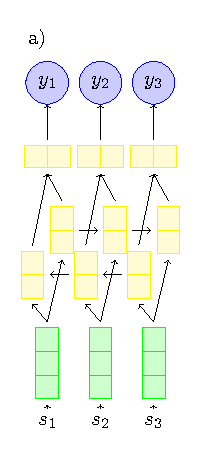
\includegraphics[scale=.65]{figures/rnnextractor.pdf}
  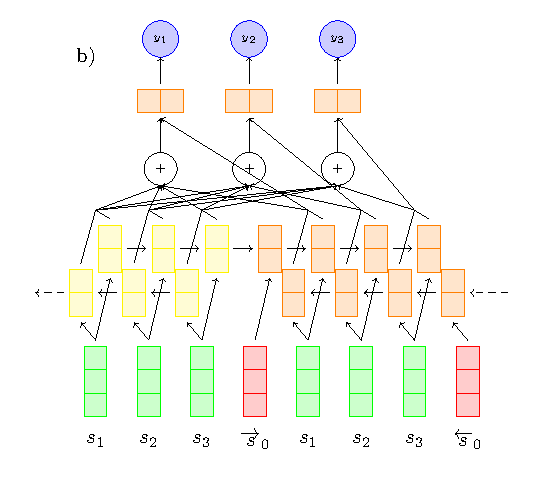
\includegraphics[scale=.65]{figures/s2s_extractor.pdf}
  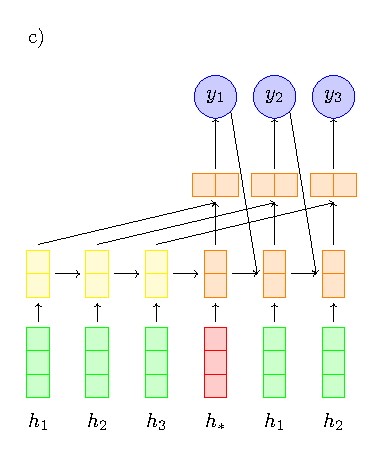
\includegraphics[scale=.65]{figures/clextractor.pdf}
  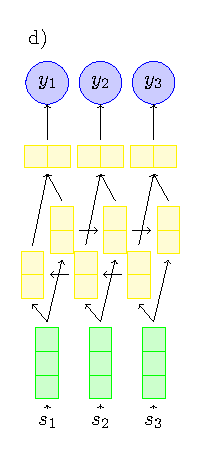
\includegraphics[scale=.65]{figures/sr_extractor.pdf}
  \caption{Sentence extractor architectures: a) RNN, b) Seq2Seq,
  c) Cheng \& Lapata, and d) SummaRunner. The $\bigoplus$ indicates 
  attention. Green repesents sentence encoder output, yellow and orange
  indicates
  extractor encoder and decoder hidden states respectively, and red indicates
  learned ``begin decoding'' embeddings. }
  \label{fig:extractors}
\end{figure*}




The goal of extractive text summarization is to select a subset of a 
document's text to use as a summary, i.e. a short gist or excerpt of the 
central content.
Typically, we impose a budget on the length of the summary in either 
words or bytes. In this work, we focus on \textit{sentence} extractive 
summarization, 
where the basic unit of extraction is a sentence and impose a word limit as 
the budget.

We model the sentence extraction task as a sequence tagging problem, 
following \cite{conroy2001text}. \hal{missing cite}
Specifically, given a document containing $\docSize$ sentences 
$\sent_1, \ldots, \sent_{\docSize}$ we generate a summary by predicting a 
corresponding label sequence $\slabel_1, \ldots, \slabel_{\docSize} 
\in \{0, 1\}^{\docSize}$, where $\slabel_i = 1$ 
indicates the $i$-th sentence is to be included in the summary.
Each sentence is itself a sequence of word embeddings 
$\sent[i] = \wordEmb[1]^{(i)}, \ldots, \wordEmb[{|\sent[i]|}]^{(i)}$ where
$|\sent[i]|$ is the length of the sentence in words.
The word budget $c \in \mathbb{N}$ 
enforces a constraint that the total summary word length 
$\sum_{i=1}^\docSize \slabel_i \cdot |\sent[i]| \le c$.






%\hal{maybe introduce some more notation here, like $s$ is a sequence of $w$s, etc. i think that might be all you need.}


For a typical deep learning model of extractive 
summarization there are two main design decisions:
%At a high level, all the models considered in this paper share the same two part structure: 
\textit{a)}  the choice of \textit{sentence encoder} 
which maps each sentence \sent[i] 
%(treated as a sequence of word embeddings) 
to an embedding $\sentEmb[i]$, 
%\hal{notation class, you used $d$ already for number of sentences} 
and 
\textit{b)} the choice of \textit{sentence extractor} 
which maps a sequence of sentence embeddings 
$\sentEmb = \sentEmb[1],\ldots, \sentEmb[\docSize]$  
to a sequence of extraction
decisions $\slabel = \slabel_1,\ldots,\slabel_{\docSize}$.
%and predicts which sentences to extract to produce the 
%extract summary. 









% anchor
\subsection{Sentence Encoders} \label{sec:senc}
\begin{figure}
  \center
  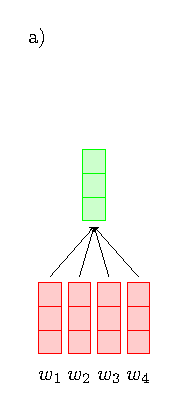
\includegraphics[scale=.7]{figures/avgsentencoder.pdf}
  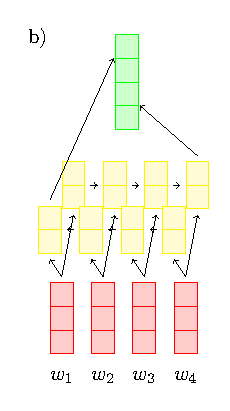
\includegraphics[scale=.7]{figures/rnnsentencoder.pdf}
  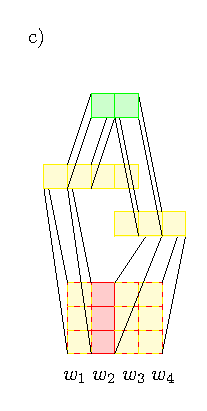
\includegraphics[scale=.7]{figures/cnnsentencoder.pdf}
  \caption{Sentence encoder architectures: a) averaging encoder, b) RNN encoder
           c) CNN encoder. Red indicates word embeddings, yellow indicates
           RNN hidden states or convolutional activations, and green 
           indicates the sentence embedding that is passed to the extractor
           module.}
    \label{fig:encoders}
\end{figure}

We treat each sentence $\sent = \{\wemb_1, \ldots, \wemb_{|\sent|}\}$ 
as a sequence of word embeddings, where $|\sent|$ is the total number of words
in the sentence. We experiment with three architectures for mapping sequences
of word embeddings to a fixed length vector: average pooling, RNNs, and CNNs.
See Figure~\ref{fig:encoders} for a diagram of the three encoders.

\textbf{Averaging Encoder} The averaging encoder (\textit{AVG}) is the simplest
method and has the added benfit of being parameter free. 
A sentence encoding is simply the average of its word embeddings: 
$\operatorname{enc}(\sent) = \frac{1}{|\sent|} \sum_{\wemb \in \sent} \wemb$.


\textbf{RNN Encoder} The \textit{RNN} sentence encoder uses the concatenation 
of the
final output states of a forward and backward RNN over the sentence's word
embeddings. We use a Gated Recurrent Unit (GRU) \cite{cho} for the RNN cell,
since it has fewer parameters than the equivalent LSTM but with similar 
performance. Formally, an \textit{RNN} sentence encoding is defined as
$\operatorname{enc}(s) = [\rSentVec_{|\sent|}; \lSentVec_1]$
where 
\begin{align} 
\rSentVec_i &= \rgru(w_i, \rSentVec_{i-1}) \\
\lSentVec_i &= \lgru(w_i, \lSentVec_{i+1}) 
\end{align}
for all $i \in 1, \ldots, |\sent|$. $\rgru$ amd $\lgru$ indicate the 
forward and backward GRUs respectively, and each have separate learned 
parameters.
The initial states $\rSentVec_0$ and $\lSentVec_{\sentSize + 1}$ are not 
learned and are set to zero vectors.

\textbf{CNN Encoder} The \textit{CNN} sentence encoder uses a series of 
convolutional feature maps to encode each sentence. This encoder is similar
to the convolutional architecture of \cite{kim} used for text classification
tasks and performs a series of ``one-dimensional'' convolutions over 
word embeddings. 
The \textit{CNN} encoder has hyperparameters
associated with the window sizes $\maxWindowSize \subset \mathcal{N}$ of the convolutional filter 
(i.e. the number of words associated with each convolution) and the number of 
feature maps $\maxFeatureMaps$ associated with each filter
(i.e. the output dimension of each 
convolution). 
The \textit{CNN} sentence encoding is computed as follows:
\begin{align}
 \specActivation_i &= \specConvBias 
    + \sum^\filterWindowSize_{j=1} \specConvWeight_j \cdot \wemb_{i + j -1}\\
  \specFeatureMap &= \max_{i\in 1,\dots, |\sent| - \filterWindowSize + 1} 
                      \relu\left(\specActivation_i\right) \\
 \senc(s) &= \left[\specFeatureMap | 
   \numFeatureMaps \in \{1, \ldots, \maxFeatureMaps\},
   \filterWindowSize \in \maxWindowSize
   \right]
\end{align}
where $\specConvBias\in\mathcal{R}$ and $\specConvWeight \in 
\mathcal{R}^{\filterWindowSize \times \wembdim}$ are learned bias and filter
weight parameters respectively, and $\relu(x) = \max(0, x)$ is the rectified
linear unit \cite{relu}.





\subsection{Sentence Extractors} \label{sec:sext}



Sentence extractors take sentence embeddings $h_{1:n}$ and produce an extract $y_{1:n}$.
The sentence extractor is essentially a discriminative 
classifier $p(\slabel_{1:n} | \sentEmb_{1:n})$.
Previous neural network approaches to sentence extraction have assumed 
an auto-regressive model, leading to a semi-Markovian
factorization of the extractor probabilities 
$p(\slabel_{1:n}|\sentEmb)=\prod_{i=1}^\docSize 
p(\slabel[i]|\slabel[<i],\sentEmb)$,
where each prediction \slabel[i] is dependent on \emph{all} 
previous \slabel[j] for
all $j < i$. We compare two such models proposed by \citet{cheng2016neural}
and \citet{nallapati2017summarunner}.
A simpler approach that does not allow interaction among the $y_{1:n}$
is to 
%\hal{a simpler approach (explain why simpler) is a fully factored representation 
  model $p(\slabel_{1:n}|\sentEmb) = \prod_{i=1}^n p(y_i|h)$, 
  which we explore in two proposed extractor models the we refer to as the RNN 
  and Seq2Seq extractors.
Implementation details for all extractors are in Appendix~\ref{app:sentextractors}.


\paragraph{Previously Proposed Sentence Extractors}
 We consider two recent state-of-the-art extractors.
%\hal{if you're hurting for space, you could probably describe these both in one paragraph, leaving off the stuff about what they use as encoders, etc., and really just making the point that they use $y<i$ to predict $yi$}

%\paragraph{Cheng \& Lapata Extractor} 
 The first, proposed by 
\citet{cheng2016neural}, %, which we refer to as the Cheng \& Lapata Extractor,
is built around a sequence-to-sequence model.
First, each sentence embedding\footnote{\citet{cheng2016neural} used an CNN sentence encoder with 
this extractor architecture; in this work we pair the Cheng \& Lapata extractor
with several different encoders.} is
fed into an encoder side RNN, with the final encoder state passed to the
first step of the decoder RNN. On the decoder side, the same sentence 
embeddings are fed as input to the decoder and decoder outputs are used to
predict each $y_i$. The decoder input is weighted by the previous extraction
probability, inducing the dependence of $y_i$ on $y_{<i}$.
See \autoref{fig:extractors}.c for a graphical layout of the extractor
and Appendix~\ref{app:clextractor} for details.

%?, but are delayed by one step and 
%?weighted by their prediction probability, i.e. at decoder step $t$,
%?$p(\slabel[t-1]|\slabel[<t-1], \sentEmb[<t-1]) \cdot \sentEmb[t-1]$\hal{why did you switch from $i$ to $t$?}
%?is fed into the decoder\hal{i don't udnerstand what this means. what op is $\cdot$?}. The decoder output at step $t$ is concatenated 
%?to the encoder output step $t$ and fed through a multi-layer perceptron
%?with one hidden layer and sigmoid unit output computing the $t$-th
%?extraction probability $p(\slabel[t]|\slabel[<t], \sentEmb[<t])$. \textcolor{red}{See Figure 2.c. for a graphical view. Full model details are presented in ??}.
%?

\citet{nallapati2017summarunner} proposed
a sentence extractor, which we refer to as the SummaRunner Extractor,
that factorizes the extraction probability into contributions 
from different sources.
First, a bidirectional RNN is run over the sentence embeddings\footnote{\citet{nallapati2017summarunner}
    use an RNN sentence encoder with 
this extractor architecture; in this work we pair the SummaRunner extractor
with different encoders. } and the output
concatenated. A representation of the whole document is made by 
averaging the RNN output. A summary representation is also constructed 
by taking the sum of the previous RNN outputs weighted by their extraction
probabilities. Extraction predictions are made using 
the RNN output at the $i$-th step, the document representation, and 
$i$-th version of the summary representation, along with factors for 
sentence location in the document. The use of the iteratively constructed
summary representation create a dependence of $y_i$ on all $y_{<i}$.
See \autoref{fig:extractors}.d for a graphical layout,
and Appendix~\ref{app:srextractor} for details.

%?A document representation $q$ is created by passing the 
%?averaged RNN output through a fully connected layer.
%?
%?Given the RNN output $z_t$ at the step $t$, the following scores are created:
%?\begin{enumerate}[nolistsep,noitemsep]
%?\item a content score $W^{(con)}z_t$,
%?\item a salience score $z_t^TW^{(sal)}q$,
%?\item a novely score $-z_t^TW^{(nov)}\tanh(g_t)$,
%?\end{enumerate}
%?where $g_t = \sum_{i=1}^{t-1} p(y_i=1|y_{<i}, h_{<i}) \cdot z_i$.
%?These scores are summed along with a bias term and a bias for sentence 
%?position and the quarter of the document\hal{what does ``the quarter of the document'' mean? sentence position quartile?} and fed through a sigmoid activation
%?to compute $p(y_t=1|y_{<t}, h_{<t})$.


\paragraph{Proposed Sentence Extractors}
We propose two sentence extractor models that 
make a stronger conditional independence 
assumption $p(\slabel|\sentEmb)=\prod_{i=1}^\docSize p(\slabel[i]|\sentEmb)$,
essentially making independent predictions conditioned on $\sentEmb$.
%In theory, our models should \hal{why should they?} perform worse because of this, however, as
%we later show, this is not the case empirically.

\paragraph{RNN Extractor}
    Our first proposed model is a very simple bidirectional
RNN based tagging model. As in the RNN sentence encoder we use a GRU cell.
The forward and backward outputs of each sentence are passed through a 
multi-layer perceptron with a logsitic sigmoid output 
to predict the probability
of extracting each sentence. 
See \autoref{fig:extractors}.a for a graphical layout,
and Appendix~\ref{app:rnnextractor} for details.


\paragraph{\sts~Extractor} One shortcoming of the RNN extractor is that long range
information from one end of the document may not easily be able to effect 
extraction probabilities of sentences at the other end. 
Our second proposed model, the \sts~extractor mitigates this problem with an 
attention 
mechanism commonly
used for neural machine translation \cite{bahdanau2014neural} and 
abstractive summarization \cite{see2017get}. 
The sentence embeddings are first
encoded by a bidirectional $\gru$. A separate decoder $\gru$ transforms each 
sentence into a query vector which attends to the encoder output. The
attention weighted encoder output and the decoder $\gru$ output are concatenated
and fed into a multi-layer percepron to compute the extraction probability.
See \autoref{fig:extractors}.b for a graphical layout,
and Appendix~\ref{app:s2sextractor} for details.

%
%We study three architectures for the sentence encoders, namely, 
%embedding averaging, RNNs, and 
%CNNs.
%We also propose two simple models for the sentence extractor and compare
%to the previously proposed extractors of 
%\citet{cheng2016neural} and \citet{nallapati2017summarunner}.
%\hal{i think it's still confusing what's new and what's not. maybe you can somewhat mark? like things with $\star$ are new and ones without are old or something?}
%The prior works differ significantly but make the same semi-Markovian
%factorization of the extraction decisions, i.e. 
%$p(\slabel|\sentEmb)=\prod_{i=1}^\docSize p(\slabel[i]|\slabel[<i],\sentEmb)$,
%where each prediction \slabel[i] is dependent on all previous \slabel[j] for
%all $j < i$.
%By contrast, our extractors make a stronger conditional independence 
%assumption $p(\slabel|\sentEmb)=\prod_{i=1}^\docSize p(\slabel[i]|\sentEmb)$,
%essentially making independent predictions conditioned on $\sentEmb$.
%In theory, our models should perform worse because of this, however, as
%we later show, this is not the case empirically.
%
%
%
%\hal{i think you might need a subsection at the end of this section with oen or two paragraphs of compare/contrast the different models, esp if details are going to appendix}
%




%%% Local Variables:
%%% mode: latex
%%% TeX-master: "dlextsum.emnlp18"
%%% End:


%\section{Models}
%At a high level, all of our models share the same two part structure: 
\textit{i) a sentence encoder} which maps an arbitrary sequence of tokens to 
an embedding $\sentvec \in \mathcal{R}^d$, and 
\textit{ii) a sentence extractor} which takes as input all of a document's 
sentence embeddings and predicts which sentences to extract to produce the 
extract summary. The sentence extractor is essentially a discriminative 
classifier $p(\slabel_1, \ldots, \slabel_{\docsize}| \sentvec_1, \ldots, \sentvec_{\docsize})$.

Depending on the architectural choices of each component we propose we 
can recover the specific implementations of \cite{cheng&lapata} and 
\cite{nallapati}, which we outline below.

\subsection{Sentence Encoders}
\begin{figure}
  \center
  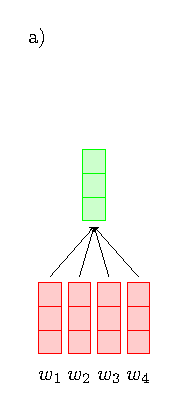
\includegraphics[scale=.7]{figures/avgsentencoder.pdf}
  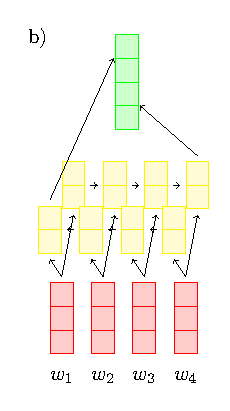
\includegraphics[scale=.7]{figures/rnnsentencoder.pdf}
  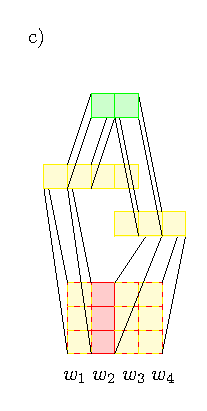
\includegraphics[scale=.7]{figures/cnnsentencoder.pdf}
  \caption{Sentence encoder architectures: a) averaging encoder, b) RNN encoder
           c) CNN encoder. Red indicates word embeddings, yellow indicates
           RNN hidden states or convolutional activations, and green 
           indicates the sentence embedding that is passed to the extractor
           module.}
    \label{fig:encoders}
\end{figure}

We treat each sentence $\sent = \{\wemb_1, \ldots, \wemb_{|\sent|}\}$ 
as a sequence of word embeddings, where $|\sent|$ is the total number of words
in the sentence. We experiment with three architectures for mapping sequences
of word embeddings to a fixed length vector: average pooling, RNNs, and CNNs.
See Figure~\ref{fig:encoders} for a diagram of the three encoders.

\textbf{Averaging Encoder} The averaging encoder (\textit{AVG}) is the simplest
method and has the added benfit of being parameter free. 
A sentence encoding is simply the average of its word embeddings: 
$\operatorname{enc}(\sent) = \frac{1}{|\sent|} \sum_{\wemb \in \sent} \wemb$.


\textbf{RNN Encoder} The \textit{RNN} sentence encoder uses the concatenation 
of the
final output states of a forward and backward RNN over the sentence's word
embeddings. We use a Gated Recurrent Unit (GRU) \cite{cho} for the RNN cell,
since it has fewer parameters than the equivalent LSTM but with similar 
performance. Formally, an \textit{RNN} sentence encoding is defined as
$\operatorname{enc}(s) = [\rSentVec_{|\sent|}; \lSentVec_1]$
where 
\begin{align} 
\rSentVec_i &= \rgru(w_i, \rSentVec_{i-1}) \\
\lSentVec_i &= \lgru(w_i, \lSentVec_{i+1}) 
\end{align}
for all $i \in 1, \ldots, |\sent|$. $\rgru$ amd $\lgru$ indicate the 
forward and backward GRUs respectively, and each have separate learned 
parameters.
The initial states $\rSentVec_0$ and $\lSentVec_{\sentSize + 1}$ are not 
learned and are set to zero vectors.

\textbf{CNN Encoder} The \textit{CNN} sentence encoder uses a series of 
convolutional feature maps to encode each sentence. This encoder is similar
to the convolutional architecture of \cite{kim} used for text classification
tasks and performs a series of ``one-dimensional'' convolutions over 
word embeddings. 
The \textit{CNN} encoder has hyperparameters
associated with the window sizes $\maxWindowSize \subset \mathcal{N}$ of the convolutional filter 
(i.e. the number of words associated with each convolution) and the number of 
feature maps $\maxFeatureMaps$ associated with each filter
(i.e. the output dimension of each 
convolution). 
The \textit{CNN} sentence encoding is computed as follows:
\begin{align}
 \specActivation_i &= \specConvBias 
    + \sum^\filterWindowSize_{j=1} \specConvWeight_j \cdot \wemb_{i + j -1}\\
  \specFeatureMap &= \max_{i\in 1,\dots, |\sent| - \filterWindowSize + 1} 
                      \relu\left(\specActivation_i\right) \\
 \senc(s) &= \left[\specFeatureMap | 
   \numFeatureMaps \in \{1, \ldots, \maxFeatureMaps\},
   \filterWindowSize \in \maxWindowSize
   \right]
\end{align}
where $\specConvBias\in\mathcal{R}$ and $\specConvWeight \in 
\mathcal{R}^{\filterWindowSize \times \wembdim}$ are learned bias and filter
weight parameters respectively, and $\relu(x) = \max(0, x)$ is the rectified
linear unit \cite{relu}.




\subsection{Sentence Extractors}
\begin{figure*}
  \center
  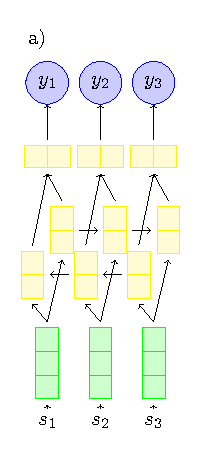
\includegraphics[scale=.7]{figures/rnnextractor.pdf}
  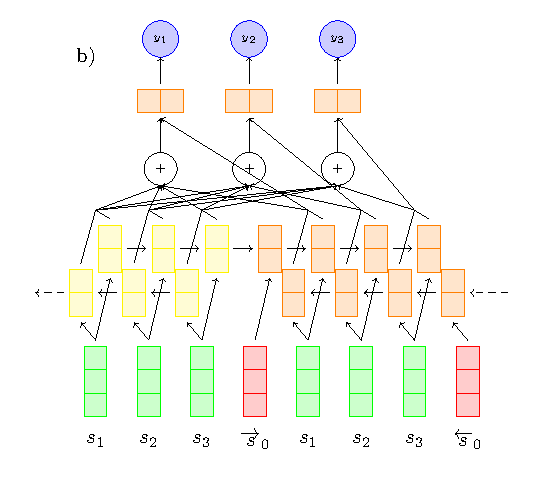
\includegraphics[scale=.7]{figures/s2s_extractor.pdf}
  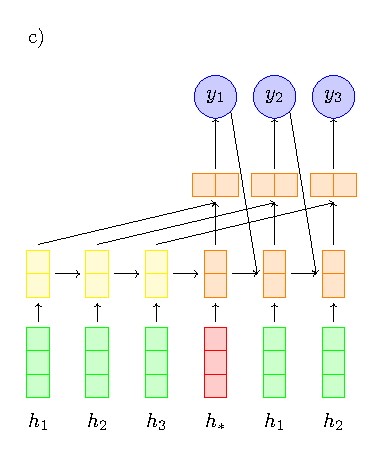
\includegraphics[scale=.7]{figures/clextractor.pdf}
  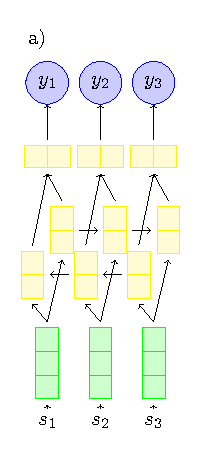
\includegraphics[scale=.7]{figures/rnnextractor.pdf}
  \caption{Sentence extractor architectures: a) \modelOneBF, b) \modelTwoBF,
            c) \baselineOneBF, and d) \baselineTwoBF. }
  \label{fig:extractors}
\end{figure*}

Given a sequence of sentence embeddings $\sentvec_i = \senc(\sent_i)$,
a sentence extractor produces a conditional distribution over the 
corresponding sentence extraction variables 
$p(\slabel_1,\ldots,\slabel_{\sentSize}|\sentvec_1, \ldots, \sentvec_{\sentSize})$.
We propose two simple recurrent neural network based sentence extractors
that make a strong conditional independence assumption over the labels
$\slabel_i$, namely
$\explicitLikelihood= \naiveLikelihood$. This stands in contrast to our 
baseline models which make a weaker assumption, \hal{this is really confusing cuz i don't think you've specified this yet, and it's still hard to understand what's new/yours and what's old/baseline.}
$\compactLikelihood = \markovLikelihood$, at the expense of greater 
computational complexity. See Figure~\ref{fig:extractors} for a diagram of the 
four sentence extractor architectures.

\textbf{RNN Extractor} Our first proposed model is a very simple bidirectional
RNN based tagging model. As in the RNN sentence encoder we use a GRU cell.
The the forward and backward outputs of each sentence are passed through a 
single layer perceptron with a logsitic sigmoid output (denoted by $\sigma$)
to predict the probability
of extracting each sentence:
\hal{i'd sugest following the same notation as before to remove the zero comment}
\begin{align}
    \rExtHidden_i &= \rgru(\sentvec_i, \rExtHidden_{i-1}) \\
   \lExtHidden_i &= \lgru(\sentvec_i, \lExtHidden_{i+1}) \\
   \logits_i &= \relu\left(U \cdot [\rExtHidden_i; \lExtHidden_i] + u \right)\\
   p(\slabel_i=1|\sentvec) &= \sigma\left(V\cdot \logits_i + v  \right)
\end{align}
for all $i \in 1, \ldots, \docsize$. $\rgru$ amd $\lgru$ indicate the 
forward and backward GRUs respectively, and each have separate learned 
parameters; $U, V$ and $u, v$ are learned weight and bias parameters.
\textcolor{red}{The initial states $\rExtHidden_0$ and $\lExtHidden_{\docsize + 1}$ are not 
learned and are set to zero vectors.}



\textbf{\sts~Extractor} One shortcoming of the RNN extractor is that long range
information from one end of the document may not easily be able to effect 
extraction probabilities of sentences at the other end. 
Our second proposed model, which we refer to as the \stsbf~extractor,
is based on the attentional sequence-to-sequence models commonly
used for neural machine translation \cite{badhanau} and 
abstractive summarization \cite{see}. The sentence embeddings are first
encoded by a bidirectional $\gru$. A separate decoder $\gru$ transforms each 
sentence into a query vector which attends to the encoder output. The
attention weighted encoder output and the decoder $\gru$ output are concatenated
and fed into a multi-layer percepron to compute the extraction probability.
Formally we have:
\begin{align}
  \rEncExtHidden_i &= \rgru_{enc}(\sentvec_i, \rEncExtHidden_{i-1}) \\
  \lEncExtHidden_i &= \lgru_{enc}(\sentvec_i, \lEncExtHidden_{i+1}) \\
  \rDecExtHidden_i &= \rgru_{dec}(\sentvec_i, \rDecExtHidden_{i-1}) \\
  \lDecExtHidden_i &= \lgru_{dec}(\sentvec_i, \lDecExtHidden_{i+1}) 
\end{align}
\begin{align}
 \decExtHidden_i = [\rDecExtHidden_i; \lDecExtHidden_i], &\;\;
 \encExtHidden_i = [\rEncExtHidden_i; \lEncExtHidden_i] 
\end{align}
\begin{align}
 \alpha_{i,j} = 
   \frac{\exp \left(\decExtHidden_i \cdot \encExtHidden_j \right)}{
   \sum_{j=1}^{\docsize}\exp\left(\decExtHidden_i \cdot \encExtHidden_j\right)}, 
& \;\; \attnExtHidden_i = \sum_{j=1}^{\docsize} \alpha_{i,j} \encExtHidden_j 
\end{align}
\begin{align}
   \logits_i = \relu\left(U \cdot [\attnExtHidden_i; \decExtHidden_i] + u \right)&\\
   p(\slabel_i=1|\sentvec) = \sigma\left(V\cdot \logits_i + v  \right),
\end{align}
for all $i \in 1, \ldots, \docsize$.
The final outputs of each encoder direction are passed to first decoder
steps; additionally, the first step of the decoder GRUs are learened 
``begin decoding'' vectors $\rDecExtHidden_0$ and $\lDecExtHidden_0$ (
see Figure~\ref{fig:extractors}.b).
Each GRU has separate learned 
parameters; $U, V$ and $u, v$ are learned weight and bias parameters.
\textcolor{red}{The initial states $\rExtHidden_0$ and $\lExtHidden_{\docsize + 1}$ are not 
learned and are set to zero vectors.}


\textbf{Cheng \& Lapata Extractor} 
We compare the previously proposed architectures to the sentence extractor
model of \cite{chenglapata}. Unlike the previous models where
sentence extraction predictions are conditionally independent given
the sentence embeddings, this model uses previous extraction probabilities to
influence later decisions. The basic architecture is a unidirectional
sequence-to-seqeunce
model defined as follows:
\begin{align}
    \encExtHidden_i &= \gru_{enc}(\sentvec_i, \encExtHidden_{i-1}) \\
    \decExtHidden_i &= \gru_{dec}(p_{i-1} \cdot \sentvec_{i-1}, \decExtHidden_{i-1}) \\
   \logits_i &= \relu\left(U \cdot [\encExtHidden_i; \decExtHidden_i] + u \right)\\
    p_i &= p(\slabel_i=1|\slabel_{<i}, \sentvec) = \sigma\left(V\cdot \logits_i + v  \right) 
\end{align}
for all $i \in 1, \ldots, \docsize$.
The final output of the encoder is passed to the first decoder
step; additionally, the first step of the decoder GRU is a learned 
``begin decoding'' vector $\decExtHidden_0$ (
see Figure~\ref{fig:extractors}.c).
Each GRU has separate learned 
parameters; $U, V$ and $u, v$ are learned weight and bias parameters.
\textcolor{red}{The initial states $\rExtHidden_0$ and $\lExtHidden_{\docsize + 1}$ are not 
learned and are set to zero vectors.}
 Note in \textcolor{red}{Equation 18} that 
the decoder side GRU input is the sentence embedding from the previous time
step weighted by its probabilitiy of extraction ($p_{i-1}$) from the 
previous step.

We refer to this extractor as the \baselineOneBF~extractor; the model 
architecture descrbied in \cite{cl} is equaivalent to the
\baselineOneBF~extractor paired with the \textit{CNN} encoder.

\hal{i'd use full names throughout if possible, so just \textbf{Chang\&Lapata} and \textbf{SummaRunner} and...}

\textbf{SummaRunner Extractor}
Our second baseline extractor is taken from \cite{nallapati}, which like the
\modelOneBF~extractor starts with a bidrectional GRU over the sentence 
embeddings 
\begin{align}
  \rEncExtHidden_i &= \rgru(\sentvec_i, \rEncExtHidden_{i-1}) \\
  \lEncExtHidden_i &= \lgru(\sentvec_i, \lEncExtHidden_{i+1}),
\end{align}
for all $i \in 1,\ldots,\docsize$. 
\textcolor{red}{The initial states $\rExtHidden_0$ and $\lExtHidden_{\docsize + 1}$ are not
learned and are set to zero vectors.}


Unlike \modelOneBF, however, it then creates a representation
of the whole document $q$ by passing the averaged GRU output states through
a fully connected layer: 
\begin{align}
q = \tanh\left(b_q + W_q\frac{1}{\docsize}\sum_{i=1}^{\docsize} [\rEncExtHidden_i; \lEncExtHidden_i] \right)
\end{align}
A concatentation of the GRU outputs at each step
are passed through a separate fully connected layer to create a 
sentence representation $z_i$, where
\begin{align}
    \extHidden_i &= \relu\left(b_z + W_z [\rEncExtHidden_i; \lEncExtHidden_i]\right).
\end{align}
The extraction probability is then determined by contributions from five 
sources,
\textit{i)} a content score $a^{(con)}_i=W_{con}\cdot z_i$, 
\textit{ii)} a salience score $a^{(sal)}_i = z_i^TW_{sal} \cdot q$ quantifying the 
similarity of the sentence to the document, 
\textit{iii)} a novelty score $a^{(nov)}_i = -z_i^TW_{nov} \cdot \tanh(g_i)$
that tracks negative similarity to a representation of the extract summary 
$g_i$,
\textit{iv)} a fine-grained position score 
$a^{(fpos)}_i = W_{fpos}\cdot p_i$ where
$p_i$ is a sentence position embedding for the $i$-th position in the document,
and \textit{v)} a coarse-grained position score 
$a^{(cpos)}_i = W_{cpos}\cdot r_i$ where
$r_i$ is a position embedding for the quarter of the document
that sentence $i$ occurs in.
The final extraction probability is the logistic sigmoid of the
sum of these terms plus a bias,
\begin{align}
    p(y_i=1|y_{<i}, h) &= \sigma\left(\begin{array}{l}
      a_i^{(con)} + a_i^{(sal)} + a_i^{(nov)} \\
  + a_i^{(fpos)}  + a_i^{(cpos)} + b \end{array}\right).
\end{align}
Finally, the iterative summary representation $g_i$ is computed as a 
sum of the previous $z_{<i}$ weighted by their extraction probabilities,
\begin{align}
g_i & = \sum_{j=1}^{i-1} p(y_j=1|y_{<j},h) \cdot z_j.
\end{align}
Note that the presence of this term induces dependence of each $y_i$ to 
all $y_{j}$ for $j < i$ similarly to the \baselineOneBF~extractor.
The combination of this extractor, which we refer to as $\baselineTwoBF$,
and the \textit{RNN} encoder is most similar to the architecture described 
in \cite{nallapati} with the principal difference that we are using the RNN
final states for the sentence representation and they used the average of
the RNN output.

%\begin{align}
%    \extHidden_i &= \relu\left(b_z + W_z [\rEncExtHidden_i; \lEncExtHidden_i]\right)
%  \end{align}
%  \begin{align*}
%      p(y_i=1|y_{<i}, h) = \sigma(& W_{con}\cdot z_i \\
%                     & + z_i^T W_{sal}\cdot q \\
%                     & -z_i^T W_{nov} \cdot \tanh(g_i) \\
%                     & + b_{rp_i}  \\
%                     & + b_{ap_i} \\
%                     & + b)     \\
%      g_j & = \sum_{i=1}^{j-1} p(y_j=1|y_{<j},h) \cdot z_j
%\end{align*}



%%% Local Variables:
%%% mode: latex
%%% TeX-master: "dlextsum.emnlp18"
%%% End:



\begin{table}

    \begin{tabular}{ f  r f r f }
      \toprule
      \textbf{Dataset} & \textbf{Train} & \textbf{Valid} & \textbf{Test} &
        \textbf{Refs} \\
      \midrule
      CNN/DM & 287,113 & 13,368 & 11,490 & 1\\
      NYT & 44,382 & 5,523 & 6,495 & 1.93\\
      DUC & 516 & 91 & 657 & 2 \\
      Reddit & 404 & 24 & 48 & 2 \\
      AMI & 98 & 19 & 20 & 1 \\
      PubMed & 21,250 & 1,250 & 2,500 & 1\\
      \bottomrule
    \end{tabular}
   \caption{Sizes of the training, validation, test splits for each dataset
   and the average number of test set human reference summaries per document.}
   \label{tab:data}
\end{table}



\begin{table*}[h]
\begin{tabular}{ccgcgcg}
    \toprule
    \multirow{2}{*}{\textbf{Extractor}} &\multirow{2}{*}{\textbf{Encoder}}  & \multicolumn{1}{g}{\textbf{CNN/DM}} & \multicolumn{1}{c}{\textbf{NYT}} & \multicolumn{1}{g}{\textbf{DUC 2002}} & \multicolumn{1}{c}{\textbf{Reddit}} & \multicolumn{1}{g}{\textbf{AMI}}\\
     &  & R-2 & R-2 & R-2 & R-2 & R-2\\
    \hline
    \multirow{3}{*}{RNN} & Avg. & 25.42 & 34.67 & 22.65 & \textbf{11.37} & \textbf{5.50}\\
     & RNN & 25.38 & 34.88 & \textbf{22.58} & \textbf{11.43} & \textbf{5.24}\\
     & CNN & 25.08 & 33.70 & \textbf{22.73} & \textbf{12.78} & 3.16\\
    \hline
    \multirow{3}{*}{Seq2Seq} & Avg. & \textbf{25.56} & \textbf{35.73} & \textbf{22.84} & \textbf{13.61} & \textbf{5.52}\\
     & RNN & 25.34 & \textbf{35.85} & 22.47 & \textbf{11.98} & \textbf{5.25}\\
     & CNN & 25.07 & 35.07 & \textbf{22.67} & \textbf{13.21} & 2.94\\
    \hline
    \multirow{3}{*}{C\&L} & Avg. & 25.29 & \textbf{35.58} & \textbf{23.11} & \textbf{13.65} & \textbf{6.12}\\
     & RNN & 25.04 & \textbf{35.84} & \textbf{23.03} & \textbf{12.62} & 4.96\\
     & CNN & 25.13 & 34.97 & \textbf{23.00} & \textbf{13.42} & 2.81\\
    \hline
    \multirow{3}{*}{SummaRunner} & Avg. & 25.44 & 35.40 & 22.28 & \textbf{13.41} & \textbf{5.63}\\
     & RNN & 25.20 & 35.47 & 22.09 & \textbf{12.51} & \textbf{5.38}\\
     & CNN & 25.00 & 34.41 & 22.22 & \textbf{12.32} & 3.16\\
    \bottomrule
\end{tabular}
  \caption{ROUGE 2 recall results across all sentence encoder/extractor pairs.
           All results are averaged over five random initializations. 
           Results that are statistically indistinguishable from the best 
           system are shown in bold face.}
  \label{tab:results}
\end{table*}


%\begin{table*}
%    \center
%    \begin{tabular}{| c | c || c | c | c | c | c | c | c | c |}
%        \hline
%         &  & \multicolumn{2}{|c|}{cnn-dailymail} & \multicolumn{2}{|c|}{nyt} & \multicolumn{2}{|c|}{duc-sds} & \multicolumn{2}{|c|}{reddit}\\
%        Extractor & Encoder & R-1 & R-2 & R-1 & R-2 & R-1 & R-2 & R-1 & R-2\\
%        \hline
%        \multirow{3}{*}{RNN} & avg & 55.3 & 25.4 & 51.4 & 34.7 & 44.1 & 22.6 & 45.2 & 11.4\\ \cline{2-10}
%         & rnn & 55.3 & 25.4 & 51.7 & 35.0 & 44.0 & 22.6 & 44.4 & 11.4\\ \cline{2-10}
%         & cnn & 54.7 & 25.1 & 50.3 & 33.7 & 44.3 & 22.7 & 47.5 & 12.7\\
%        \hline
%        \multirow{3}{*}{Seq2Seq} & avg & \textbf{55.6} & \textbf{25.6} & 52.5 & 35.7 & 44.4 & 22.8 & \textbf{49.1} & \textbf{13.6}\\ \cline{2-10}
%                                 & rnn & 55.2 & 25.3 & 52.5 & \textbf{35.9} & 43.8 & 22.5 & 45.4 & 12.1\\ \cline{2-10}
%         & cnn & 54.8 & 25.1 & 51.7 & 35.1 & 44.0 & 22.7 & 46.8 & 13.1\\
%        \hline
%        \multirow{3}{*}{C\&L} & avg & 55.1 & 25.3 & 52.3 & 35.6 & \textbf{44.8} & \textbf{23.1} & 48.3 & 13.6\\ \cline{2-10}
%         & rnn & 54.8 & 25.0 & 52.5 & 35.8 & 44.5 & 23.0 & 46.3 & 12.6\\ \cline{2-10}
%         & cnn & 55.0 & 25.1 & 51.5 & 35.0 & 44.5 & 23.0 & 46.9 & 13.4\\
%        \hline
%        \multirow{3}{*}{SR} & avg & 55.3 & 25.4 & 52.1 & 35.4 & 44.0 & 22.3 & 48.8 & 13.4\\ \cline{2-10}
%         & rnn & 55.0 & 25.2 & 52.1 & 35.5 & 43.6 & 22.1 & 46.5 & 12.6\\ \cline{2-10}
%         & cnn & 54.6 & 25.0 & 51.0 & 34.4 & 43.6 & 22.2 & 46.6 & 12.3\\
%        \hline
%    \end{tabular}
%\end{table*}


\section{Datasets}
\label{sec:datasets}
We perform our experiments across six corpora from varying domains to 
understand how different biases within each domain can affect content 
selection. The corpora come from the news domain
(CNN-DailyMail, New York Times, DUC), personal narratives domain (Reddit),
workplace meetings (AMI), and medical journal articles (PubMed). See 
\autoref{tab:data} for dataset statistics.


\paragraph{CNN-DailyMail} We use the preprocessing and training, validation, 
and test splits
of \cite{see2017get}.
This corpus is a mix of news on different topics including politics,
sports, and entertainment.

\paragraph{New York Times}The New York Times (NYT) corpus \cite{sandhaus2008new} contains
 two types of abstracts for a subset of its articles. The first summary is
an abstract \textcolor{red}{produced by an archival librarian} and the 
second is an online teaser meant to elicit a viewer on the webpage to
click to read more. From this collection we take all articles that have 
a combined summary length of at least 100 words
%\hal{i'm not sure what you mean here. are you concatenating the two summaries? if so, say so. is that a little weird tho?}. This collection
%includes both straight newswire as well as opinion and long-form journalism.
We create training, validation, and test splits by partitioning on dates;
we use the year 2005 as the validation data, with training and test partitions
including documents before and after 2005 respectively.
%yielding $44,382$ training, $5,523$ validation, and $6,495$ test documents.

\paragraph{DUC} We use the single document summarization data from the 2001
and 2002
Document Understanding Conferences (DUC) \cite{over2002introduction}. We split the 2001 data into training
and validation splits and reserve the 2002 data for testing.
%, resulting in
%516/91/657 documents for training, validation, and test respectively. 
%The test set has two or three human abstracts roughly 100 words in length per 
%articles.}

\paragraph{AMI} The AMI corpus \cite{carletta2005ami} 
is collection of real and staged office meetings
annotated with text transcriptions, along with abstractive
summaries. We use the prescribed splits. 
%to get 98/19/20 training, validation,
%and test examples with one human abstract summary per meeting. 
%We ignore any speaker information since we are primarily
%interested in studying content selection in a domain agnostic way.
%The summaries are about 290 words long on average and so we target this length
%for summary generation. \hal{a) you don't need braces around paragraph text. b) this is the only place you mention task stuff rather than dataset stuff. mabye move target length information to the experiments section?}


\paragraph{Reddit} \citet{ouyang2017crowd} collected a corpus of personal 
    stories shared
 on Reddit\footnote{\url{www.reddit.com}} along with multiple extractive 
 and abstractive summaries. %These stories are relatively short compared
 %to the other corpora with an average sentence length of ??. 
%\kathy{Why didn't you use theirs?}
% We created our own train, validation, and test splits resulting in 
%404/24/48 documents respectively. 
%}

\paragraph{PubMed}{We created a corpus of 25,000 randomly samples 
    medical journal articles from the PubMed Open Access 
    Subset\footnote{\url{https://www.ncbi.nlm.nih.gov/pmc/tools/openftlist/}}.
    We only included articles if they were at least 1000 words long and 
    had an abstract of at least 50 words in length.
We used the article abstracts as the ground truth human summaries.}
\hal{maybe mention this in the intro with a footnote about data release? we've recently used statements like the following in a footnote:
  \textbf{Code and data release:} Upon publication, all code and pre-processing scripts will be released under an MIT (or more liberal) license; all data will be made available after publication when allowed by original licenses.}

\subsection{Ground Truth Extract Summaries}
Since we do not typically have ground truth extract summaries from which to
create the labels $\slabel_i$, we construct gold label sequences 
by greedily optimizing ROUGE-1, as follows.
%?\begin{algorithm}[H]
%?    \KwData{$I = \{\sent[1], \ldots, \sent[n]\}$, word budget $c$} 
%?    empty summary $\summary = \emptyset$\\
%?    $y_i = 0 \quad \forall i \in 1, \ldots, n$ \\
%?    \While{$\sum_{\sent[i] \in \summary} |\sent[i]| \le c \;$}{
%?        $\hat{\sent} = {\argmax}_{ \sent[i] \in I \setminus \summary} \rouge(\summary \cup \sent[i])$\\
%?  \eIf{$\rouge(\summary \cup \hat{\sent}) > \rouge(\summary)$}{
%?       $\summary \gets \summary \cup \hat{\sent}$
%?   }{\textbf{break}\\}
%?                                       }
%?$y_i \gets 1 $ if $s_i \in S \; \forall i \in 1, \ldots, n$\\ 
%?\KwResult{$y = y_1,\ldots y_n$}
%?%                                        \caption{How to write algorithms}
%?\end{algorithm}


\begin{algorithmic}

\State $I = \{\sent[1], \ldots, \sent[n]\};\quad y_i = 0 \quad \forall i \in 1, \ldots, n$
\State    empty summary $\summary = \emptyset$; ~~word budget $c$
\While{$\sum_{\sent[i] \in \summary} |\sent[i]| \le c \;$} 
\State $\hat{i} = {\argmax}_{ i \in \{j \in [n]| \sent[j] \notin \summary\}} \rouge(\summary \cup \sent[i])$
\If {$\rouge(\summary \cup \sent[\hat{i}]) > \rouge(\summary)$}
\State $\summary \gets \summary \cup \sent[\hat{i}]; \quad y_{\hat{i}} = 1$
        \Else
        \State \textbf{break} 
       \EndIf
\EndWhile
\State \Return $y=y_1, \ldots, y_n$
\end{algorithmic}

%\begin{enumerate}
%\item Start with an empty summary $\summary = 
%\null \emptyset$ and word limit $c$. 
%\item while $\sum_{i \in \summary} |\sent[i]| \le c$:
%    \begin{enumerate}
%        \item $\hat{\sent} = {\argmax}_{ i \in [\docSize] \setminus \summary} \operatorname{ROUGE}(\summary \cup \sent[i])$
%\item if $\operatorname{ROUGE}(\summary \cup \hat{\sent}) > \operatorname{ROUGE}(\summary)$
%    \begin{enumerate}
%        \item $\summary \leftarrow \summary \cup \hat{\sent}$
%    \end{enumerate}
%\item else break
%
%%to $\summary$ 
%\end{enumerate}
%\item return $y_i =\begin{cases} 1 & \textrm{if $i \in S$}\\ 0 & \textrm{otherwise} \end{cases}$ for all $i \in [n]$.
%\end{enumerate}
%stopping when the ROUGE-1 score no longer increases or the 
%length budget is reached\hal{what does this mean. does it mean that if the $\hat s$ that's selected puts you over length limit then you stop, or is it that you stop when there are no more sentences that you can cram in? and what if adding $\hat s$ doesn't make rouge go up?}. 
We choose to optimize for ROUGE-1 rather than 
ROUGE-2 similarly to other optimization based approaches to summarization 
\textcolor{red}{
\cite{durrett2016learning,sipos2012large,nallapati2017summarunner} which found this
be the easier optimization target.}



%%% Local Variables:
%%% mode: latex
%%% TeX-master: "dlextsum.emnlp18"
%%% End:


\begin{table*}[h]
\center
\begin{tabular}{ccgcgcg}
    \toprule
    \multirow{2}{*}{\textbf{Extractor}} &\multirow{2}{*}{\textbf{Embeddings}}  & \multicolumn{1}{g}{\textbf{CNN/DM}} & \multicolumn{1}{c}{\textbf{NYT}} & \multicolumn{1}{g}{\textbf{DUC 2002}} & \multicolumn{1}{c}{\textbf{Reddit}} & \multicolumn{1}{g}{\textbf{AMI}}\\
     &  & R-2 & R-2 & R-2 & R-2 & R-2\\
    \hline
    \multirow{2}{*}{RNN} & Fixed & \textbf{25.42} & \textbf{34.67} & \textbf{22.65} & \textbf{11.37} & \textbf{5.50}\\
     & Learned & 25.21 & 34.31 & \textbf{22.60} & \textbf{11.30} & \textbf{5.30}\\
    \hline
    \multirow{2}{*}{Seq2Seq} & Fixed & \textbf{25.56} & \textbf{35.73} & \textbf{22.84} & \textbf{13.61} & 5.52\\
     & Learned & 25.34 & \textbf{35.65} & \textbf{22.88} & \textbf{13.78} & \textbf{5.79}\\
    \hline
    \multirow{2}{*}{C\&L} & Fixed & \textbf{25.29} & \textbf{35.58} & \textbf{23.11} & \textbf{13.65} & \textbf{6.12}\\
     & Learned & 24.95 & 35.41 & \textbf{22.98} & \textbf{13.39} & \textbf{6.16}\\
    \hline
    \multirow{2}{*}{SummaRunner} & Fixed & \textbf{25.44} & \textbf{35.40} & \textbf{22.28} & \textbf{13.41} & \textbf{5.63}\\
     & Learned & 25.11 & 35.20 & \textbf{22.15} & 12.64 & \textbf{5.85}\\
    \bottomrule
\end{tabular}



\caption{ROUGE-2 recall across sentence extractors
    when using learned or pretrained embeddings. In both cases embeddings
    are initialized with pretrained GloVe embeddings. All results are 
averaged from five random initializations. All extractors use the averaging 
sentence encoder. When both learned and unlearned settings are bolded,
there is no signifcant performance difference.}
\label{tab:embeddings}
\end{table*}

%\begin{table*}
%\center
%\begin{tabular}{| c | c || c | c | c | c | c | c | c | c |}
%\hline
%  &   & \multicolumn{2}{|c|}{cnn-dailymail} & \multicolumn{2}{|c|}{nyt} & \multicolumn{2}{|c|}{duc-sds} & \multicolumn{2}{|c|}{reddit} \\
%system & embeddings & R1 & R2  & R1 & R2  & R1 & R2  & R1 & R2  \\
%\hline
%\multirow{2}{*}{RNN} & fixed & 55.3 & 25.4 & 51.4 & 34.7 & 44.1 & 22.6 & 45.2 & 11.4\\ \cline{2-10}
% & learned & 55.1 & 25.2 & 51.1 & 34.3 & 44.1 & 22.6 & 45.3 & 11.3\\
%\hline
%\multirow{2}{*}{Seq2Seq} & fixed & 55.6 & 25.6 & 52.5 & 35.7 & 44.4 & 22.8 & 49.1 & 13.6\\ \cline{2-10}
% & learned & 55.2 & 25.3 & 52.4 & 35.7 & 44.5 & 22.9 & 49.4 & 13.8\\
%\hline
%\multirow{2}{*}{C\&L} & fixed & 55.1 & 25.3 & 52.3 & 35.6 & 44.8 & 23.1 & 48.3 & 13.6\\ \cline{2-10}
% & learned & 54.8 & 25.0 & 52.1 & 35.4 & 44.6 & 23.0 & 48.6 & 13.5\\
%\hline
%\multirow{2}{*}{SummaRunner} & fixed & 55.3 & 25.4 & 52.1 & 35.4 & 44.0 & 22.3 & 48.8 & 13.4\\ \cline{2-10}
% & learned & 55.0 & 25.1 & 52.0 & 35.2 & 43.8 & 22.1 & 47.8 & 12.6\\
%\hline
%\end{tabular}
%\caption{ROUGE 1 and 2 recall results across different sentence extractors
%    when using learned or pretrained embeddings. In both cases embeddings
%    are initialized with pretrained GloVe embeddings. All results are 
%averaged from five random initializations. All extractors use the averaging 
%sentence encoder.}
%\label{tab:embeddings}
%\end{table*}

\begin{table*}[ht]
\center
\begin{tabular}{cgcgcgc}
    \toprule
    \multirow{1}{*}{\textbf{Ablation}}  & \multicolumn{1}{g}{\textbf{CNN/DM}} & \multicolumn{1}{c}{\textbf{NYT}} & \multicolumn{1}{g}{\textbf{DUC}} & \multicolumn{1}{c}{\textbf{Reddit}} & \multicolumn{1}{g}{\textbf{AMI}} & \multicolumn{1}{c}{\textbf{PubMed}}\\
    \hline
    all words & \textbf{25.4}\textsuperscript{~} ~~~~~~~ & \textbf{34.7}\textsuperscript{~} ~~~~~~~~& 22.7\textsuperscript{~} ~~~~~~~~& \textbf{11.4}\textsuperscript{~} ~~~~~~~~& 5.5\textsuperscript{~} ~~~~~~~~~& \textbf{17.0}\textsuperscript{~} ~~~~~~~ \\
    -nouns & 25.3\textsuperscript{$\dagger$} \footnotesize{(0.1)}& 34.3\textsuperscript{$\dagger$} \footnotesize{(0.4)}& 22.3\textsuperscript{$\dagger$} ~\footnotesize{(0.4)}& 10.3\textsuperscript{$\dagger$} \footnotesize{(1.1)} & 3.8\textsuperscript{$\dagger$} \footnotesize{(1.7)}& 15.7\textsuperscript{$\dagger$} \footnotesize{(1.3)}\\
    -verbs & 25.3\textsuperscript{$\dagger$} \footnotesize{(0.1)}& 34.4\textsuperscript{$\dagger$} \footnotesize{(0.3)} & 22.4\textsuperscript{$\dagger$} ~\footnotesize{(0.3)}& 10.8\textsuperscript{~} ~\footnotesize{(0.6)} & 5.8\textsuperscript{~} \footnotesize{(-0.3)} & 16.6\textsuperscript{$\dagger$} \footnotesize{(0.4)}\\
    -adj/adv & 25.3\textsuperscript{$\dagger$} \footnotesize{(0.1)}& 34.4\textsuperscript{$\dagger$} \footnotesize{(0.3)} & 22.5\textsuperscript{~} ~\footnotesize{(0.2)} & ~~9.5\textsuperscript{$\dagger$} \footnotesize{(1.9)} & 5.4\textsuperscript{~} ~\footnotesize{(0.1)} & 16.8\textsuperscript{$\dagger$} \footnotesize{(0.2)}\\
    -function & 25.2\textsuperscript{$\dagger$} \footnotesize{(0.2)} & 34.5\textsuperscript{$\dagger$} \footnotesize{(0.2)} & \textbf{22.9}\textsuperscript{$\dagger$} \footnotesize{(-0.2)} & 10.3\textsuperscript{$\dagger$} \footnotesize{(1.1)}& \textbf{6.3}\textsuperscript{$\dagger$} \footnotesize{(-0.8)}& 16.6\textsuperscript{$\dagger$} \footnotesize{(0.4)}\\
    \bottomrule
\end{tabular}

\caption{ROUGE-2 recall after removing nouns, verbs, adjectives/adverbs, and 
    function words. Ablations are
    performed using the averaging sentence encoder and the RNN
extractor. 
Bold indicates best performing system. $\dagger$ indicates significant 
difference with the non-ablated system. Difference in score from \textit{all words} shown in parenthesis.}
\label{tab:ablations}
\end{table*}

\begin{table*}[h]
\center
\begin{tabular}{llgcgcg}
    \toprule
    \multirow{2}{*}{\textbf{Extractor}} &\multirow{2}{*}{\textbf{Sentence Order}}  & \multicolumn{1}{g}{\textbf{CNN/DM}} & \multicolumn{1}{c}{\textbf{NYT}} & \multicolumn{1}{g}{\textbf{DUC 2002}} & \multicolumn{1}{c}{\textbf{Reddit}} & \multicolumn{1}{g}{\textbf{AMI}}\\
     &  & R-2 & R-2 & R-2 & R-2 & R-2\\
    \hline
    \multirow{2}{*}{RNN} & In-Order & \textbf{25.42} & \textbf{34.67} & \textbf{22.65} & \textbf{11.37} & \textbf{5.50}\\
     & Shuffled & 22.80 & 24.96 & 18.24 & \textbf{11.83} & \textbf{5.70}\\
    \hline
    \multirow{2}{*}{Seq2Seq} & In-Order & \textbf{25.56} & \textbf{35.73} & \textbf{22.84} & \textbf{13.61} & 5.52\\
     & Shuffled & 21.66 & 25.61 & 21.21 & \textbf{13.45} & \textbf{5.98}\\
    \bottomrule
\end{tabular}

\caption{ROUGE-2 recall using models trained on in-order and shuffled
documents. All extractors use the averaging sentence encoder. 
Table shows average results of five random initializations.
When both in-order and shuffled settings are bolded,
there is no signifcant performance difference.
}
\label{tab:shuffle}
\end{table*}


%\begin{table*}
%\center
%\begin{tabular}{| c | c || c | c | c | c | c | c |}
%\hline
%  &   & \multicolumn{2}{|c|}{nyt} & \multicolumn{2}{|c|}{duc-sds} & \multicolumn{2}{|c|}{reddit} \\
%Extractor & sentence order & R1 & R2  & R1 & R2  & R1 & R2 \\ 
%\hline
%\multirow{2}{*}{RNN} & in-order & 51.4 & 34.7 & 44.1 & 22.6 & 45.2 & 11.4\\ \cline{2-8}
% & shuffled & 41.9 & 25.0 & 39.7 & 18.2 & 45.1 & 11.9\\
%\hline
%\multirow{2}{*}{Seq2Seq} & in-order & 52.5 & 35.7 & 44.4 & 22.8 & 49.1 & 13.6\\ \cline{2-8}
% & shuffled & 42.6 & 25.6 & 42.9 & 21.2 & 48.7 & 13.6\\
%\hline
%\end{tabular}
%\caption{ROUGE 1 and 2 recall using models trained on in-order and shuffled
%documents. All extractors use the averaging sentence encoder. 
%Table shows average results of five random initializations.}
%\label{tab:shuffle}
%\end{table*}



\section{Experiments} \label{sec:exps}
\kathy{Could Lapata or Nallapati criticize your choice of parameters here as not being the same as what they used? (Note that I don't know what they used but it seems like a possible criticism.)}
We train all models to minimize the weighted negative log likelihood
\[\mathcal{L} = -\sum_{s,y\in \mathcal{D}} \sum_{i=1}^\docSize \omega(y_i) \log p\left(y_i|y_{<i},
\operatorname{enc}(\sent)\right)\]
over the training data $\mathcal{D}$
using stochastic gradient descent with the ADAM optimizer
\hal{maybe just say $\omega(0)=1$ and $\omega(1) = N_0/N_1$ where $N_y$ is the number of examples with label $y$.}
\cite{kingma2014adam}. The term 
\[ \omega(y_i)=\begin{cases}
\frac{\sum_{y_j} \mathbbm{1}\{y_j = 0 \}}{ \sum_{y_j} \mathbbm{1}\{y_j = 1 \}  } & \textrm{if $y_i=1$} \\ 1 & \textrm{otherwise}  \end{cases} \] 
        upweights
    positive examples proportionally to the ratio of negative to positive
    examples in the training data in order to compensate for the sparsity
    of the positive class.
\kathy{Could you say how you arrived at these settings? Is any one system penalized by the use of uniform settings?}
    We use a learning rate of .0001 and a dropout rate of .25 for all dropout
    layers. We also employ gradient clipping ($-5 < \nabla_\theta < 5$). 
    We train for a maximum of 30 epochs and the best
    model is selected with early stopping on the validation set according
    to ROUGE-2 recall. All experiments are repeated with five random
    initializations. Weight matrix parameters are initialized using 
    Xavier initialization with the normal distribution 
    \cite{glorot2010understanding} and bias terms are set to 0.
    Unless specified, word embeddings are initialized 
    using pretrained GloVe embeddings \cite{pennington2014glove} and we do 
    not update them during training. Unknown words are mapped to a zero 
    embedding.
    We use a batch size of 32 for all datasets except AMI and PubMed for
    which we use sizes two and four respectively. 
\kathy{why? Say.}
    For the Cheng \& Lapata model, we train for half of the maximum epochs 
    with teacher forcing, i.e. we set $p_i = 1$
    if $y_i = 1$ in the gold data and 0 otherwise 
    when computing the decoder input 
    $p_i \cdot \sentEmb[i]$; we revert to the true model probability 
    during the second half training.

\subsection{Ground Truth Extract Summaries}
    \hal{i feel like this should go before the optimizer dtails}
Since we do not typically have ground truth extract summaries from which to
create the labels $\slabel_i$, we construct gold label sequences 
by greedily optimizing ROUGE-1. Starting with an empty summary $\summary = 
\null \emptyset$, we add the sentence $\hat{\sent} = 
{\argmax}_{ \sent \in \{\sent_1, \ldots, \sent_{\docsize}\},
\; \sent \notin \summary} \operatorname{ROUGE-1}(\summary \cup \sent)$
to $\summary$ stopping when the ROUGE-1 score no longer increases or the 
length budget is reached. We choose to optimize for ROUGE-1 rather than 
ROUGE-2 similarly to other optimization based approaches to summarization 
\textcolor{red}{
\cite{durrett2016learning,sipos2012large,nallapati2017summarunner} which found this
be the easier optimization target.}


\hal{do you say anywhere how you do significance testing and what significance level you use?}




\paragraph{Extractor/Encoder Comparions}{
In our main experiment, we compare our proposed 
sentence extractors, RNN and Seq2Seq,
to those of Cheng \& Lapata and SummaRunner.
We test all possible sentence extractor/encoder pairs across all the datasets
described in Section~\ref{sec:datasets}.} 
%We choose ROUGE-2
%recall as our main evaluation metric since it has the strongest correlation
%to human content selection decisions.

\kathy{Save all results for results section. I deleted your sentence.}
\hal{i agree with kathy. put all the results together. be specific about what questions you're asking and then how you framed them as an experiment and then what the answer is. i think i'd just remove all this stuff here.}
%In most cases, the averaging encoder performance was as good or better than
%the RNN and CNN encoders, we use only the averaging encoder for the remainder
%of the experiments.

\paragraph{Word Embedding Learning}{To futher understand how word 
embeddings 
can
effect model performance we also compared extractors when embeddings 
are updated during training. Both fixed and learned embedding variants are 
initialized with GloVe embeddings. When learning embeddings, words occurring 
three or fewer times in the training data are mapped to a learned unkown
token.}

\paragraph{POS Tag Ablation}{Additionally, we ran ablation experiments
using part-of-speech (POS) tags. 
All datasets were automatically tagged using
the SpaCy POS tagger \footnote{https://github.com/explosion/spaCy}.   
\kathy{I'm still curious what would happen if you separately removed all conjunction tags and later remaining POS.}
We experimented with selectively removing 
\begin{itemize}
    \item nouns (NOUN and PROPN tags), 
    \item verbs (VERB, PART, and AUX tags), 
    \item adjectives/adverbs (ADJ and ADV tags), 
    \item numerical expressions (NUM and SYM tags), and 
    \item miscellaneous words (ADP, CONJ, CCONJ, DET, INTJ, and SCONJ tags)
\end{itemize}
from each sentece. 
The embeddings of removed words were replaced with a zero vector,
preserving the order and position of the non-ablated words in the sentence.
}

\textbf{Document Shuffling} In examining the outputs of the models, we found
most of the selected sentences in the news domain came from the lead paragraph
of the document. This is despite the fact that there is a long tail of 
sentence extractions from later in the document in the ground truth extract 
summaries. Because this lead bias is so strong, it is questionable whether
the models are learning to identify important content or just find the start
of the document. We perform a series of sentence order experiments where 
each document's sentences are randomly shuffled during training. We then
%KM - I think below should be shuffled. I changed.
%CK - models are trained on shuffled data but evaluated on in order models.
%evaluate each model performance on the unshuffled test data, comparing to 
evaluate each model performance on the unshuffled test data, comparing to 
the original unshuffled models. 

%We are also interested in the effect of lead bias. It is well known that the first few sentences of a news article, often referred to as the lead, make a good summary, and this is most commonly used as the default baseline in single document summarization. This lead bias is such a strong learning signal that the learned models almost always extract sentences from the lead despite the ground truth labeling containing a significant portion of positive labels later in the document. This begs the question, are we learning a robust model of sentence salience or simply identifying linguistic style features that are indicative of the lead?

%To better understand this phenomenon, 




%%% Local Variables:
%%% mode: latex
%%% TeX-master: "dlextsum.emnlp18"
%%% End:


\begin{table*}[ht]
    \footnotesize
\centering
  \begin{tabular}{p{24em} p{24em}}
\toprule
Hurricane Gilbert swept toward the Dominican Republic Sunday, and the 
   Civil Defense alerted its heavily populated south coast to prepare 
   for high winds, heavy rains and high seas.                         
The storm was approaching from the southeast with sustained winds of  
   75 mph gusting to 92 mph.                                          
An estimated 100,000 people live in the province, including 70,000 in 
   the city of Barahona, about 125 miles west of Santo Domingo.       
\textbf{On Saturday, Hurricane Florence was downgraded to a tropical storm and
   its remnants pushed inland from the U.S. Gulf Coast.}               
Tropical Storm Gilbert formed in the eastern Caribbean and            
   strengthened into a hurricane Saturday night.  
&
Hurricane Gilbert swept toward the Dominican Republic Sunday, and the 
   Civil Defense alerted its heavily populated south coast to prepare 
   for high winds, heavy rains and high seas.                         
The storm was approaching from the southeast with sustained winds of  
   75 mph gusting to 92 mph.                                          
An estimated 100,000 people live in the province, including 70,000 in 
   the city of Barahona, about 125 miles west of Santo Domingo.       
Tropical Storm Gilbert formed in the eastern Caribbean and            
   strengthened into a hurricane Saturday night.                      
\textbf{Strong winds associated with the Gilbert brought coastal flooding,    
   strong southeast winds and up to 12 feet feet to Puerto Rico's     
   south coast.}   \\
\bottomrule
\end{tabular}
\caption{Example output of Seq2Seq extractor (left) and Cheng 
\& Lapata Extractor (right). This is a typical example, where only one
 sentence is different between the two (shown in bold). }
\label{tab:output}
\end{table*}

\subsection{Results} 


The results of our main experiment comparing 
the different extractors/encoders are shown in 
Table~\ref{tab:results}.
Overall, we find no major advantage when using the CNN and RNN sentence
encoders. The best performing encoder/extractor pair uses the averaging 
encoder (\textcolor{red}{4 out of 5 datasets}) or the differences 
are not statistically significant. When only comparing within the 
same extractor choice,  the averaging encoder is the better choice
in 14 of 20 cases. 
\hal{i wonder if it would be worth adding another ``average performance metric'' column to \autoref{tab:results}.
  i'm thinking have ``Average $\Delta$-Best'' meaning how far (on average across the datasets) is this setting from the best setting available on that dataset.
  so since the best numbers are: 25.56, 35.85, 23.11, 13.65, 5.63
  and the first row numbers are: 25.42, 34.67, 22.65, 11.37, 5.50
  then the deltas are:            0.14,  1.18,  0.46,  2.28, 0.13
  the the average delta is 0.84 (assuming my math is right)
  there's an argument to do multiplicative, in which case
  the multipliers for first row:  0.99,  0.97,  0.98,  0.83, 0.97
  and the average is 0.95
  either way this gives a quick way to make comparisons between rows. you could do the same for the other tables too.}

  \hal{in some of the tables you list R-2 as headers even though all the numbers are R-2. just put that in the caption.}


When looking at extractors, the Seq2Seq extractor is either part of 
the best performing system (\textcolor{red}{2 out of 5} datasets) or is not 
statistically distinguishable from the best extractor. 

Overall, on the news domain, the differences are quite small with the 
differences between worst and best systems on the CNN/DM dataset 
spanning only .56 of a ROUGE point. While there is more performance variability
 in the non-news domains, there is less distinction among systems: all systems
are statistically indistinguishable from the best system on Reddit
and every extractor has at least one configuration that is indistinguishable
from the best system on the AMI corpus.\hal{this is probably at least partially because of test set size. maybe mention this.}





%?\textcolor{red}{Overall we find that the \modelTwoBF~extractor achieves the 
%?best ROUGE scores on three out of four domains (STILL RUNNING ON AMI AND PUBMED). 
%?However, most
%?differences are not signficant. (Need to discuss stat sig and how to show it).}
%?On the larger CNN-DailyMail dataset, especially, 
%?differences are quite smail across all extractor/encoder pairs.
%?The \baselineOneBF~extractor achieves the best performance on the DUC 2002
%?dataset. It is disappointing that the \baselineOneBF~and \baselineTwoBF~based 
%?models do not gain any apparent advantage in conditioning on previous 
%?sentence selection decisions; this result suggests the need to improve
%?the representation of the summary as it is being constructed iteratively.
%?
%?\textbf{Choice of Encoder} We also find there to be no major advantage 
%?between the different sentence encoders. \textcolor{red}{In most cases,
%?there is no statistical significance between the averaging encoder and either
%?the RNN or CNN encoders.} 

%The lack of differentiation amongst the different encoders concerning; one
%would assume learning with the appropriate structure would be helpful.
%The results of next 




\paragraph{Word Embedding Learning}{

Table~\ref{tab:embeddings} shows ROUGE recall
when using fixed or updated word embeddings. 
\textcolor{red}{In all but one case,
fixed embeddings are as good or better than the learned embeddings.}
This is a somewhat surprising finding, and suggests that our models\hal{why is it surprising?}
cannot extract much generalizable learning signal from the content than what 
is already present from initialization. 
The AMI corpus is an exception here where learning does lead to small
performance boosts, however, only in the Seq2Seq extractor is this diference 
significant. The language of this corpus is quite different from the 
data that the GloVe embeddings were trained on and so it makes sense 
that  there would be more benefit to learning word representations; one
explanation for only seeing modest improvements is purely the small size
of the dataset \textcolor{red}{(NOTE TO CK -- expect learning to help on pubmed)}. \hal{yes, the dataset size is certainly an issue here. probably worth pointing this out. also when you learned the embeddings, did you initialize to pretrained embeddings? did you regularize toward them?}


}

\begin{table*}[ht]
\center
\begin{tabular}{cgcgcgc}
    \toprule
    \multirow{1}{*}{\textbf{Ablation}}  & \multicolumn{1}{g}{\textbf{CNN/DM}} & \multicolumn{1}{c}{\textbf{NYT}} & \multicolumn{1}{g}{\textbf{DUC}} & \multicolumn{1}{c}{\textbf{Reddit}} & \multicolumn{1}{g}{\textbf{AMI}} & \multicolumn{1}{c}{\textbf{PubMed}}\\
    \hline
    all words & \textbf{25.4}\textsuperscript{~} ~~~~~~~ & \textbf{34.7}\textsuperscript{~} ~~~~~~~~& 22.7\textsuperscript{~} ~~~~~~~~& \textbf{11.4}\textsuperscript{~} ~~~~~~~~& 5.5\textsuperscript{~} ~~~~~~~~~& \textbf{17.0}\textsuperscript{~} ~~~~~~~ \\
    -nouns & 25.3\textsuperscript{$\dagger$} \footnotesize{(0.1)}& 34.3\textsuperscript{$\dagger$} \footnotesize{(0.4)}& 22.3\textsuperscript{$\dagger$} ~\footnotesize{(0.4)}& 10.3\textsuperscript{$\dagger$} \footnotesize{(1.1)} & 3.8\textsuperscript{$\dagger$} \footnotesize{(1.7)}& 15.7\textsuperscript{$\dagger$} \footnotesize{(1.3)}\\
    -verbs & 25.3\textsuperscript{$\dagger$} \footnotesize{(0.1)}& 34.4\textsuperscript{$\dagger$} \footnotesize{(0.3)} & 22.4\textsuperscript{$\dagger$} ~\footnotesize{(0.3)}& 10.8\textsuperscript{~} ~\footnotesize{(0.6)} & 5.8\textsuperscript{~} \footnotesize{(-0.3)} & 16.6\textsuperscript{$\dagger$} \footnotesize{(0.4)}\\
    -adj/adv & 25.3\textsuperscript{$\dagger$} \footnotesize{(0.1)}& 34.4\textsuperscript{$\dagger$} \footnotesize{(0.3)} & 22.5\textsuperscript{~} ~\footnotesize{(0.2)} & ~~9.5\textsuperscript{$\dagger$} \footnotesize{(1.9)} & 5.4\textsuperscript{~} ~\footnotesize{(0.1)} & 16.8\textsuperscript{$\dagger$} \footnotesize{(0.2)}\\
    -function & 25.2\textsuperscript{$\dagger$} \footnotesize{(0.2)} & 34.5\textsuperscript{$\dagger$} \footnotesize{(0.2)} & \textbf{22.9}\textsuperscript{$\dagger$} \footnotesize{(-0.2)} & 10.3\textsuperscript{$\dagger$} \footnotesize{(1.1)}& \textbf{6.3}\textsuperscript{$\dagger$} \footnotesize{(-0.8)}& 16.6\textsuperscript{$\dagger$} \footnotesize{(0.4)}\\
    \bottomrule
\end{tabular}

\caption{ROUGE-2 recall after removing nouns, verbs, adjectives/adverbs, and 
    function words. Ablations are
    performed using the averaging sentence encoder and the RNN
extractor. 
Bold indicates best performing system. $\dagger$ indicates significant 
difference with the non-ablated system. Difference in score from \textit{all words} shown in parenthesis.}
\label{tab:ablations}
\end{table*}


\textbf{POS Ablation} Table~\ref{tab:ablations} shows the results of the POS
tag ablation experiments. \hal{i'd label the rows as ``all words'' and then ``- nouns'', ``- verbs'', etc. also use paragraph not textbf :P.}
While removing any word class from the representation generally hurts \hal{is this removed at train and test or just test?}
performance (with statistical significance) on the news domains,
the absolute values of the differences are quite small 
(.18 on CNN/DM, .41 on NYT, .3 on DUC) suggesting that the model's predictions
are not overly dependent on any particular word types.\hal{i'm not sure i agree. if it's significant it's significant, no?} 
On the non-news datasets, the ablations have a larger effect 
(max differences are 1.89 on Reddit, 2.56 on AMI). \hal{if you're mentioning absolute differences here i'd do that in the tables too}
Removing the content words leads to the largest drop on AMI.
Removing adjectives and adverbs leads to the largest drop on Reddit,
suggesting the intensifiers and descriptive words are useful for 
identifying important content in personal narratives.
Curiously, 
removing the miscellaneous POS class yields a significant improvement
on DUC 2002 and AMI.


%The newswire domain does not appear to be sensative
%to these ablations; this suggests that the models are still able to identify
%the lead section of the document with the remaining word classes \textcolor{red}{(Verify this with histogram analysis)}. 
%The Reddit domain, which is not lead biased, is significantly effected.
%Notably, removing adjectives and adverbs results in a 1.8 point drop 
%in ROUGE-2 recall. 

\begin{table*}[h]
\center
\begin{tabular}{llgcgcg}
    \toprule
    \multirow{2}{*}{\textbf{Extractor}} &\multirow{2}{*}{\textbf{Sentence Order}}  & \multicolumn{1}{g}{\textbf{CNN/DM}} & \multicolumn{1}{c}{\textbf{NYT}} & \multicolumn{1}{g}{\textbf{DUC 2002}} & \multicolumn{1}{c}{\textbf{Reddit}} & \multicolumn{1}{g}{\textbf{AMI}}\\
     &  & R-2 & R-2 & R-2 & R-2 & R-2\\
    \hline
    \multirow{2}{*}{RNN} & In-Order & \textbf{25.42} & \textbf{34.67} & \textbf{22.65} & \textbf{11.37} & \textbf{5.50}\\
     & Shuffled & 22.80 & 24.96 & 18.24 & \textbf{11.83} & \textbf{5.70}\\
    \hline
    \multirow{2}{*}{Seq2Seq} & In-Order & \textbf{25.56} & \textbf{35.73} & \textbf{22.84} & \textbf{13.61} & 5.52\\
     & Shuffled & 21.66 & 25.61 & 21.21 & \textbf{13.45} & \textbf{5.98}\\
    \bottomrule
\end{tabular}

\caption{ROUGE-2 recall using models trained on in-order and shuffled
documents. All extractors use the averaging sentence encoder. 
Table shows average results of five random initializations.
When both in-order and shuffled settings are bolded,
there is no signifcant performance difference.
}
\label{tab:shuffle}
\end{table*}


%\begin{table*}
%\center
%\begin{tabular}{| c | c || c | c | c | c | c | c |}
%\hline
%  &   & \multicolumn{2}{|c|}{nyt} & \multicolumn{2}{|c|}{duc-sds} & \multicolumn{2}{|c|}{reddit} \\
%Extractor & sentence order & R1 & R2  & R1 & R2  & R1 & R2 \\ 
%\hline
%\multirow{2}{*}{RNN} & in-order & 51.4 & 34.7 & 44.1 & 22.6 & 45.2 & 11.4\\ \cline{2-8}
% & shuffled & 41.9 & 25.0 & 39.7 & 18.2 & 45.1 & 11.9\\
%\hline
%\multirow{2}{*}{Seq2Seq} & in-order & 52.5 & 35.7 & 44.4 & 22.8 & 49.1 & 13.6\\ \cline{2-8}
% & shuffled & 42.6 & 25.6 & 42.9 & 21.2 & 48.7 & 13.6\\
%\hline
%\end{tabular}
%\caption{ROUGE 1 and 2 recall using models trained on in-order and shuffled
%documents. All extractors use the averaging sentence encoder. 
%Table shows average results of five random initializations.}
%\label{tab:shuffle}
%\end{table*}

\textbf{Document Shuffling} Table~\ref{tab:shuffle} shows the results
of our shuffling experiments. 
The newswire domain suffer a significant drop in performance 
when the document order is shuffled. \textcolor{red}{By comparison, there is no significant difference between the shuffled and in-order models on 
the Reddit domain, and shuffling actually improves performance on the AMI}.\hal{what about in the cross-domain setting?}





\begin{table*}
\begin{tabular}{lllrrrrr}
%\toprule
    &     &          & cnn-dailymail &      nyt &  duc-sds &   reddit &     ami \\
    &     &          &            R2 &       R2 &       R2 &       R2 &      R2 \\
Source Dataset & Extractor & Doc Order &               &          &          &          &         \\
%\midrule
cnn-dailymail & RNN & In-Order &       25.4172 &  32.6914 &  22.7538 &  14.5222 &  4.0718 \\
nyt & RNN & In-Order &       24.1500 &  34.6666 &  22.9564 &  11.2408 &  4.2336 \\
duc-sds & RNN & In-Order &       23.5106 &  32.2476 &  22.6520 &  12.3368 &  3.0092 \\
reddit & RNN & In-Order &       23.0648 &  27.9204 &  20.6258 &  11.3940 &  2.5646 \\
ami & RNN & In-Order &        9.6806 &   7.7956 &  12.6174 &  10.7048 &  5.4958 \\
cnn-dailymail & RNN & Shuffled &       22.8038 &  25.5584 &  21.3410 &  \textbf{14.7008} &  3.4252 \\
nyt & RNN & Shuffled &       17.5148 &  24.9578 &  20.6572 &  10.4836 &  3.8924 \\
duc-sds & RNN & Shuffled &       16.9730 &  18.6806 &  18.2378 &  11.7118 &  3.2894 \\
reddit & RNN & Shuffled &       22.7654 &  27.7366 &  20.5632 &  11.8348 &  2.6030 \\
ami & RNN & Shuffled &        9.9302 &   8.2276 &  12.7670 &  10.2996 &  5.7002 \\
cnn-dailymail & Seq2Seq & In-Order &       \textbf{25.5560} &  32.5312 &  22.7042 &  14.3916 &  3.8886 \\
nyt & Seq2Seq & In-Order &       24.4888 &  \textbf{35.7280} &  \textbf{23.0692} &  10.7674 &  3.5056 \\
duc-sds & Seq2Seq & In-Order &       24.3412 &  32.7244 &  22.8384 &  12.9758 &  3.5844 \\
reddit & Seq2Seq & In-Order &       18.7552 &  23.7096 &  19.8706 &  13.7194 &  3.0072 \\
ami & Seq2Seq & In-Order &       12.1790 &   9.7512 &  13.7606 &   9.9028 &  5.5226 \\
cnn-dailymail & Seq2Seq & Shuffled &       21.6618 &  22.6544 &  19.9770 &  14.0084 &  3.8104 \\
nyt & Seq2Seq & Shuffled &       18.2358 &  25.6094 &  20.5528 &  12.0216 &  3.6208 \\
duc-sds & Seq2Seq & Shuffled &       19.6998 &  25.5266 &  21.2116 &  12.0884 &  3.4744 \\
reddit & Seq2Seq & Shuffled &       19.4136 &  23.8588 &  19.8218 &  13.4550 &  2.8182 \\
ami & Seq2Seq & Shuffled &       13.5160 &  13.3164 &  15.6102 &  10.2888 &  \textbf{5.9806} \\
%\bottomrule
\end{tabular}



\end{table*}


%%% Local Variables:
%%% mode: latex
%%% TeX-master: "dlextsum.emnlp18"
%%% End:




\section{Discussion}

\begin{table*}
\centering
  \begin{tabular}{p{20em} p{20em}}
\toprule
Hurricane Gilbert swept toward the Dominican Republic Sunday, and the 
   Civil Defense alerted its heavily populated south coast to prepare 
   for high winds, heavy rains and high seas.                         
The storm was approaching from the southeast with sustained winds of  
   75 mph gusting to 92 mph.                                          
An estimated 100,000 people live in the province, including 70,000 in 
   the city of Barahona, about 125 miles west of Santo Domingo.       
\textbf{On Saturday, Hurricane Florence was downgraded to a tropical storm and
   its remnants pushed inland from the U.S. Gulf Coast.}               
Tropical Storm Gilbert formed in the eastern Caribbean and            
   strengthened into a hurricane Saturday night.  
&
Hurricane Gilbert swept toward the Dominican Republic Sunday, and the 
   Civil Defense alerted its heavily populated south coast to prepare 
   for high winds, heavy rains and high seas.                         
The storm was approaching from the southeast with sustained winds of  
   75 mph gusting to 92 mph.                                          
An estimated 100,000 people live in the province, including 70,000 in 
   the city of Barahona, about 125 miles west of Santo Domingo.       
Tropical Storm Gilbert formed in the eastern Caribbean and            
   strengthened into a hurricane Saturday night.                      
\textbf{Strong winds associated with the Gilbert brought coastal flooding,    
   strong southeast winds and up to 12 feet feet to Puerto Rico's     
   south coast.}   \\
\bottomrule
\end{tabular}
\caption{Example output of Seq2Seq extractor (left) and Cheng 
\& Lapata Extractor (right). This is a typical example, where only one
 sentence is different between the two (show in bold). }
\label{tab:output}
\end{table*}

Learning in the news domain is severely inhibited by the lead bias. 
The output of all systems is highly similar to each other and to the lead 
baseline. Using the averaging encoder, the Seq2Seq and Cheng \& Lapata
extractors share 87.8\% of output sentences on average on the CNN/DM data,
with similar numbers for the other news domains (see \autoref{tab:output}
for a typical example).  
Also on CNN/DM, 58\% of the Seq2Seq with averaging encoder outputs sentences also occurring
in the lead summary, with similar numbers for DUC, NYT, and Reddit. Shuffling
reduces lead overlap to 35.2\% but the overall system performance drops
    significantly.
    The relative robustness of the news domain to POS ablation also suggests
    suggests that models are mostly learning to recognize the stylistic 
    features unique to the beggining of the article, and not the content.
    Additionally, drop in performance when learning word embeddings on 
    the news domain suggests that word embeddings alone do not provide 
    very generalizable content features compared to recognizing the lead.

The picture is rosier for non-news summarization where POS ablation leads
to larger performance differences and shuffling either does not inhibit content
selection significantly or leads to modest gains. In order to learn better
word-level representations on these domains will likely require much
larger corpora, somthing which might remain unlikely for personal narratives
and meetings.



The lack of distinction amongst sentence encoders is interesting because 
it echoes findings in the generic sentence embedding literature 
where word embedding averaging is frustratingly difficult to 
outperform  \cite{wieting2015towards,arora2016simple,wieting2017revisiting}.
The inability to learn useful sentence representations is also 
borne out in the 
SummaRunner model, where there are explicit similarity computations
between document or summary representations and sentence embeddings;
these computations do not seem to add much to the performance as the 
Cheng \& Lapata and Seq2Seq models which lack these features generally
perform as well or better.
Furthermore, the Cheng \& Lapata and SummaRunner extractors both construct
a history of previous selection decisions to inform future choices but this
does not seem to significantly improve performance over the Seq2Seq extractor 
which does not, suggesting that we need to rethink or find novel forms 
of sentence representation for the summarization task.


A manual examination of the outputs revealed some interesting failure modes
although in general it was hard to discern clear patterns of behaviour 
other than lead bias. On the news domain, the models consistently learned 
to ignore quoted material in the lead, as often the quotes provide
color to the story but are unlikely to be included in the summary (e.g.\textit{``It was like somebody slugging a punching bag.''}). 
This behavior was most likely triggered by the presence of quotes, as the
quote attributions, which were often tokenized as separate sentences,
would subsequently be included in the summary despite also not containing 
much information 
(e.g. \textit{Gil Clark of the National Hurricane Center said Thursday}).




The Reddit corpus was particularly challenging as often there was no concise
way to extractively represent the story. Authors often inserted a 
fairly brief summary of the story, either at the end or beginning, but
this was so abstractive as to not have much overlap with the reference
summaries. For example, the first sentence, \textit{I took a dog off the street, and she changed my grandparent's lives}, has little overlap with the reference
\textit{The dog I found for my grandparents still gets really excited to see
me whenever I come to visit}, but is still functionally a reasonable 
summary of the story. These ``micro summaries'' do not seem to be 
consistently found by any summarization model. 






\section{Conclusion}
We have presented an empirical study of deep learning based content selection
algorithms for summarization. Our findings suggest such models face stark limitations on their ability to learn robust features for this task and that 
more work is needed on sentence representation for summarization.



\bibliography{emnlp2018}
\bibliographystyle{acl_natbib_nourl}

\newpage
\onecolumn
\appendix

\begin{centering}
  \Large
  Supplementary Material For:\\
  Content Selection in Deep Learning Models of Summarization\\

\end{centering}

  \section{Details on Sentence Encoders} \label{app:sentencoders}

  We use 200 dimenional word embeddings \wordEmb[i] in all models.

\subsection{Details on RNN Encoder} \label{app:rnnencoder}
  
Under the \textit{RNN} encoder, a sentence embedding is defined as
$\sentEmb = [\rSentEmb[\sentSize]; \lSentEmb[1]]$
where 
\begin{align} 
  \rSentEmb[0] = \mathbf{0} &;\quad 
       \rSentEmb[i] = \rgru(\wordEmb[i], \rSentEmb[i-1]) \\
  \lSentEmb[\sentSize + 1] = \mathbf{0} &;\quad 
       \lSentEmb[i] = \lgru(\wordEmb[i], \lSentEmb[i+1]),
%\lSentVec_i &= \lgru(w_i, \lSentVec_{i+1}) 
\end{align}
and $\rgru$ amd $\lgru$ indicate the 
forward and backward GRUs respectively, each with separate 
parameters.

\subsection{Details on CNN Encoder} \label{app:cnnencoder}
The \textit{CNN} encoder has hyperparameters
associated with the window sizes $\maxWindowSize \subset \mathcal{N}$ of the convolutional filter 
(i.e. the number of words associated with each convolution) and the number of 
feature maps $\maxFeatureMaps$ associated with each filter
(i.e. the output dimension of each 
convolution). 
The \textit{CNN} sentence embedding $\sentEmb$ is computed as follows:
\begin{align}
 \specActivation_i &= \specConvBias 
    + \sum^\filterWindowSize_{j=1} \specConvWeight_j \cdot \wemb_{i + j -1}\\
  \specFeatureMap &= \max_{i\in 1,\dots, |\sent| - \filterWindowSize + 1} 
                      \relu\left(\specActivation_i\right) \\
 \sentEmb &= \left[\specFeatureMap | 
   \numFeatureMaps \in \{1, \ldots, \maxFeatureMaps\},
   \filterWindowSize \in \maxWindowSize
   \right]
\end{align}
where $\specConvBias\in\mathcal{R}$ and $\specConvWeight \in 
\mathcal{R}^{\filterWindowSize \times \wordEmbSize}$ are learned bias and filter
weight parameters respectively, and $\relu(x) = \max(0, x)$ is the rectified
linear unit activation.

\section{Details on Sentence Extractors} \label{app:sentextractors}
\subsection{Details on RNN Extractor} \label{app:rnnextractor}
\begin{align}
    \rExtHidden_0 = \mathbf{0};&\quad   \rExtHidden_i = \rgru(\sentEmb[i], \rExtHidden_{i-1}) \\
    \lExtHidden_{\docSize + 1} = \mathbf{0};&\quad    \lExtHidden_i = \lgru(\sentEmb[i], \lExtHidden_{i+1}) \\
   \logits_i &= \relu\left(U \cdot [\rExtHidden_i; \lExtHidden_i] + u \right)\\
   p(\slabel_i=1|\sentvec) &= \sigma\left(V\cdot \logits_i + v  \right)
\end{align}
where $\rgru$ and $\lgru$ indicate the 
forward and backward GRUs respectively, and each have separate learned 
parameters; $U, V$ and $u, v$ are learned weight and bias parameters.

\subsection{Details on Seq2Seq Extrator} \label{app:s2sextractor}
\begin{align}
    \rEncExtHidden_0 = \textbf{0}&;\quad \rEncExtHidden_i = \rgru_{enc}(\sentEmb[i], \rEncExtHidden_{i-1}) \\
    \lEncExtHidden_{\docSize + 1} = \textbf{0}&;\quad  \lEncExtHidden_i = \lgru_{enc}(\sentEmb[i], \lEncExtHidden_{i+1}) \\
    \rDecExtHidden_i &= \rgru_{dec}(\sentEmb[i], \rDecExtHidden_{i-1}) \\
    \lDecExtHidden_i &= \lgru_{dec}(\sentEmb[i], \lDecExtHidden_{i+1}) 
\end{align}
\begin{align}
 \decExtHidden_i = [\rDecExtHidden_i; \lDecExtHidden_i], &\;\;
 \encExtHidden_i = [\rEncExtHidden_i; \lEncExtHidden_i] 
\end{align}
\begin{align}
 \alpha_{i,j} = 
   \frac{\exp \left(\decExtHidden_i \cdot \encExtHidden_j \right)}{
   \sum_{j=1}^{\docSize}\exp\left(\decExtHidden_i \cdot \encExtHidden_j\right)}, 
& \;\; \attnExtHidden_i = \sum_{j=1}^{\docSize} \alpha_{i,j} \encExtHidden_j 
\end{align}
\begin{align}
   \logits_i = \relu\left(U \cdot [\attnExtHidden_i; \decExtHidden_i] + u \right)&\\
   p(\slabel_i=1|\sentvec) = \sigma\left(V\cdot \logits_i + v  \right).
\end{align}
The final outputs of each encoder direction are passed to the first decoder
steps; additionally, the first step of the decoder GRUs are learned 
``begin decoding'' vectors $\rDecExtHidden_0$ and $\lDecExtHidden_0$ 
(see Figure~\ref{fig:extractors}.b).
Each GRU has separate learned 
parameters; $U, V$ and $u, v$ are learned weight and bias parameters.

\subsection{Details on Cheng \& Lapata Extractor.} \label{app:clextractor}
The basic architecture is a unidirectional
sequence-to-sequence
model defined as follows:
\begin{align}
    \encExtHidden_0 = \textbf{0};&\quad   \encExtHidden_i = \gru_{enc}(\sentvec_i, \encExtHidden_{i-1}) \\
    \decExtHidden_1 &= \gru_{dec}(\sentEmb[*], \encExtHidden_{\docSize}) \\
    \decExtHidden_i &= \gru_{dec}(p_{i-1} \cdot \sentvec_{i-1}, \decExtHidden_{i-1}) \label{eq:cl1} \\
   \logits_i &= \relu\left(U \cdot [\encExtHidden_i; \decExtHidden_i] + u \right)\\
    p_i = p(\slabel_i&=1|\slabel_{<i}, \sentvec) = \sigma\left(V\cdot \logits_i + v  \right) 
\end{align}
where \sentEmb[*] is a learned ``begin decoding'' sentence embedding
(see Figure~\ref{fig:extractors}.c).
Each GRU has separate learned 
parameters; $U, V$ and $u, v$ are learned weight and bias parameters.
Note in Equation~\ref{eq:cl1} that 
the decoder side GRU input is the sentence embedding from the previous time
step weighted by its probabilitiy of extraction ($p_{i-1}$) from the 
previous step, inducing dependence of each output $y_i$ on all previous 
outputs $y_{<i}$.

%\kathy{In many ways the Cheng and Lapata architecture looks simpler than yours. Can you indicate here why it is more complicated? Is it because of the number of learned parameters?}

Note that in the original paper, the Cheng \& Lapata extractor was paired 
with
a \textit{CNN} sentence encoder, but in this work we experiment with a variety
of sentence encoders.

\subsection{Details on SummaRunner Extractor.} \label{app:srextractor}
Like the
RNN~extractor it starts with a bidrectional GRU over the sentence 
embeddings 
\begin{align}
    \rEncExtHidden_0 = \textbf{0}&;\quad \rEncExtHidden_i = \rgru(\sentvec_i, \rEncExtHidden_{i-1}) \\
    \lEncExtHidden_{\docSize + 1} = \textbf{0}&;\quad \lEncExtHidden_i = \lgru(\sentvec_i, \lEncExtHidden_{i+1}),
\end{align}

It then creates a representation
of the whole document $q$ by passing the averaged GRU output states through
a fully connected layer: 
\begin{align}
q = \tanh\left(b_q + W_q\frac{1}{\docSize}\sum_{i=1}^{\docSize} [\rEncExtHidden_i; \lEncExtHidden_i] \right)
\end{align}
A concatentation of the GRU outputs at each step
are passed through a separate fully connected layer to create a 
sentence representation $z_i$, where
\begin{align}
    \extHidden_i &= \relu\left(b_z + W_z [\rEncExtHidden_i; \lEncExtHidden_i]\right).
\end{align}
The extraction probability is then determined by contributions from five 
sources:
\begin{align}
    \textit{content} &\quad a^{(con)}_i=W^{(con)} z_i, \\
    \textit{salience}&\quad a^{(sal)}_i = z_i^TW^{(sal)} q, \\
    \textit{novelty}&\quad a^{(nov)}_i = -z_i^TW^{(nov)} \tanh(g_i), \label{eq:srnov} \\
    \textit{position}&\quad a^{(pos)}_i = W^{(pos)} l_i, \\
    \textit{quartile}&\quad a^{(qrt)}_i = W^{(qrt)} r_i,
\end{align}
where $l_i$ and $r_i$ are embeddings associated with the $i$-th sentence
position and the quarter of the document containing sentence $i$ respectively.
In Equation~\ref{eq:srnov}, $g_i$ is an iterative summary representation 
computed as the
sum of the previous $z_{<i}$ weighted by their extraction probabilities,
\begin{align}
g_i & = \sum_{j=1}^{i-1} p(y_j=1|y_{<j},h) \cdot z_j.
\end{align}
Note that the presence of this term induces dependence of each 
$\slabel_i$ to 
all $\slabel_{<i}$ similarly to the Cheng \& Lapata extractor.

The final extraction probability is the logistic sigmoid of the
sum of these terms plus a bias,
\begin{align}
    p(y_i=1|y_{<i}, h) &= \sigma\left(\begin{array}{l}
      a_i^{(con)} + a_i^{(sal)} + a_i^{(nov)} \\
  + a_i^{(pos)}  + a_i^{(qrt)} + b \end{array}\right).
\end{align}
The weight matrices $W_q$, $W_z$, $W^{(con)}$, $W^{(sal)}$, $W^{(nov)}$, $W^{(pos)}$,
$W^{(qrt)}$ and bias terms $b_q$, $b_z$, and $b$ are learned parameters;
The GRUs have separate learned parameters.

Note that in the original paper, the SummaRunner extractor was paired 
with
an \textit{RNN} sentence encoder, but in this work we experiment with a variety
of sentence encoders.


\section{Ground Truth Extract Summary Algorithm} \label{app:oracle}
\begin{algorithmic}

    \State \textbf{data:} $I = \{\sent[1], \ldots, \sent[n]\}$;
    \State $y_i = 0 \quad \forall i \in 1, \ldots, n$;
\State    empty summary $\summary = \emptyset$; ~~word budget $c$
\While{$\sum_{\sent[i] \in \summary} |\sent[i]| \le c \;$} 
\State $\hat{i} = {\argmax}_{ i \in \{j \in [n]| \sent[j] \notin \summary\}} \rouge(\summary \cup \{\sent[i]\})$
\If {$\rouge(\summary \cup \{ \sent[\hat{i}] \} ) > \rouge(\summary)$}
\State $\summary \gets \summary \cup \{ \sent[\hat{i}] \}; \quad y_{\hat{i}} = 1$
        \Else
        \State \textbf{break} 
       \EndIf
\EndWhile
\State \Return $y=y_1, \ldots, y_n$
\end{algorithmic}
\hal{is this right? this could yield something longer than the budget size because what if the last step selects a really long sentence.
  i think you want the argmax over $\{j \in [n] - S : \sum \dots \leq c\}$ to make things brief maybe define $\textit{len}$ to be the current summary length? or $\textit{len}(S)$? also minor quibble but i like $S \cup \{s_i\}$ better than without the braces. CK this is what I did. I saved all summary length constraint for the eval, e.g. rouge just chops things off at 100 words. Not ideal but in practice i think it helps to have more to predict, ie less positive label sparseness, since we are no where near accurately predicting these labels anyway.}



\section{Optimizer and initialization settings.} \label{app:optset}

    We use a learning rate of .0001 and a dropout rate of .25 for all dropout
    layers. We also employ gradient clipping ($-5 < \nabla_\theta < 5$).
Weight matrix parameters are initialized using 
    Xavier initialization with the normal distribution 
    \cite{glorot2010understanding} and bias terms are set to 0.
    We use a batch size of 32 for all datasets except AMI and PubMed, which
    are often longer and consume more memory, for
    which we use sizes two and four respectively.
%\kathy{why? Say.}
    For the Cheng \& Lapata model, we train for half of the maximum epochs 
    with teacher forcing, i.e. we set $p_i = 1$
    if $y_i = 1$ in the gold data and 0 otherwise 
    when computing the decoder input 
    $p_i \cdot \sentEmb[i]$; we revert to the true model probability 
    during the second half training.
\hal{i feel like this paragraph was produced by a summarization algorithm run on the state of Chris' brain :P --- that is to say, it's not super coherant. maybe reorder things so that they are in order of train/apply/eval or something? right now i'm not sure what matters and what doesn't matter. also so-called teacher forcing breaks the definition of log likelihood above, but maybe that's fine.}






\makeappendix

\end{document}
